%% $RCSfile: proj_proposal.tex,v $
%% $Revision: 1.2 $
%% $Date: 2010/04/23 02:40:16 $
%% $Author: kevin $

\documentclass[11pt, a4paper, twoside, openright]{report}
\usepackage{float}
\usepackage{url}
\usepackage{harvard}
\usepackage{multirow}
\usepackage{array}
\usepackage{amsmath}
\usepackage{graphicx}
\usepackage{booktables}
\usepackage[toc,page]{appendix}
\usepackage{algorithm}
\usepackage[options]{algorithm2e}

\graphicspath{{figures/}}

\newfloat{fig}{thp}{lof}[chapter]
\floatname{fig}{Figure}

\title{Priority Based Traffic Control}
\author{James McCann}

\usepackage[image,ecs]{vuwproject} 
\supervisor{Paul Teal}
\otherdegree{Bachelor of Engineering (Hons)}

\date{}

\begin{document}

\frontmatter

\begin{abstract}

The rising ubiquity of internet connected devices and wireless networks offers a bright future for intelligent transport systems in urban environments. By equipping individual vehicles with wireless devices capable of communicating with traffic signal controllers, adaptive traffic control schemes can be used to prioritise traffic flows, minimise delay based on traffic priority, and reduce the rising costs of congestion within our urban networks.

The Priority Based Traffic Control system (PBTC) is a tool for simulating the opportunities allowed by a fully connected traffic fleet. By establishing wireless communication with vehicles approaching a controlled intersection and estimating the operational stopping cost and delay cost for each vehicle, the PBTC system can adapt to local traffic conditions in real time, minimising the congestion costs incurred by road users. Lookahead estimation allows a signal controller to extend green time dynamically to further reduce the cost associated with phase changes. 

This paper presents the PBTC system architecture, methods used to estimate and minimise the costs of delaying approaching traffic at a controlled intersection, and results of evaluation against vehicle actuated and adaptive control methods.
  
\end{abstract}

\maketitle

%\tableofcontents

% we want a list of the figures we defined
%\listof{fig}{Figures}

\mainmatter

\chapter{Introduction}

Transportation is fundamental to the modern global economy, encouraging growth and job creation, trade, and quality of life. The success of road transportation and steady increase in the number of individual vehicles in use has resulted in an ongoing strain on societies to provide infrastructure capable of satisfying demand. 

Widespread utilisation of road transport for commercial and private use has lead to significant traffic congestion in densely populated, urban environments as demand outstrips the capacity of roading networks \cite{euro2011whitepaper,papa2003review}. As the complexity of road networks increases, so too does the need for control systems to safely and efficiently manage access to shared road by competing flows of traffic. 

Intersections with signal controls allow competing traffic flows to independently make use of the limited capacity of intersecting sections of  two or more roads. To avoid collisions, allowing traffic to flow through a controlled intersection requires stopping all competing traffic flows also demanding the intersection. As a result, controlled intersection delay is one of the most significant causes of congestion costs in urban road networks.

\section {Motivations}

Urban congestion is a significant problem facing the New Zealand transportation industry. In 2013, an independent consultation commissioned by the New Zealand Transport Agency (NZTA) found that the increase in transport cost due to congestion within Auckland City could be as high as 1.2 billion dollars annually when compared to freely flowing traffic \cite{wallis2013costs}. Modeling the cost of individual vehicle journeys through controlled intersections in a road network could allow for traffic systems to make efforts to minimise these congestion costs.

% where does this sentence go?
The New Zealand Ministry of Transport (MoT) 2008 transport strategy identifies affordability and efficiency as two primary goals of transportation development over the next three decades and recommends future congestion management strategies should make more efficient use of existing network capacity without the need to add expensive new infrastructure. Improving the effectiveness of traffic signal controls at road intersections has potential benefits for all controlled intersections in New Zealand, at significantly lower costs than infrastructure changes \cite{mot2008strategy}.

\section{Problem}

Modern intersection signal controllers seek to minimise delay by responding to vehicle demand at each incoming link. Adaptive traffic control systems, such as the Sydney Coordinated Adaptive Traffic Control System (SCATS), operated at all controlled intersections on New Zealand cities and highways; adaptively increment phase plans in response to near-real time traffic conditions and are successful for reducing delay within high demand road networks \cite{lowrie1982scats,akcelik1998evaluation,wolshon1999scats}.

Existing traffic control systems, such as SCATS, are limited to minimising the number of queued cars or average delay at an intersection. When an approaching vehicle is stopped at a controlled intersection, a cost is absorbed by the occupants or owners of the vehicle. Costs incurred may be caused by the physical characteristics of a vehicle, for example: a stopped vehicle must use more fuel to accelerate back to a cruise speed; or by the impact of the delay on the vehicle occupants in terms of added commuting time. To reduce the costs of congestion on road networks, traffic control systems should be designed to consider the potential costs of each vehicle within the network.

As an example of this problem, consider a common "cross-roads" intersection, with two competing approaches. If a large, commercial freight vehicle running late for a ferry and a small family car returning home from a shopping trip are approaching the intersection on two competing roads, who should be given right of way? There is significantly more cost incurred if the truck is forced to stop at the intersection, including cost of fuel required to accelerate and the potential of being late for the ferry and missing a shipment. In a traditional vehicle actuated or adaptive traffic control system, there is no guarantee on who will be given the opportunity to pass first. The traffic controller is not influenced by the potential costs of stopping approaching traffic and, depending on the current signal phase timing, it is likely that both vehicles are forced to stop, or the truck is forced to stop. 

This project presents a new method for adaptive traffic control that considers individual vehicles approaching or waiting at an intersection based on a dynamically calculated \emph{priority} value, calculated using properties of each vehicle that can be communicated to a traffic controller using wireless devices embedded in vehicles. Vehicular Ad-hoc Networks (VANETs) that allow vehicles to communicate with other vehicles and infrastructure using short-range wireless technologies are an area of increasing research and offer new opportunities for adaptive traffic signal control \cite{adaptive2007grad,nadeem2004trafficview,yang2004vehicle}.

\section{Objectives}

Three primary objectives were identified as core to this project. The chapters following will discuss each of the project developments and contributions with respect to the objectives identified here.

Firstly, design of a priority model to estimate the costs incurred by the journey of an individual vehicle through a road network. This objective is required to establish a basis for estimating and minimising cost values for a priority-aware traffic control system. A priority model is expected to assign a relative measure of the priority of every vehicle in a road network, based on the cost of stopping or delaying the vehicle. Vehicle priority modelling allows for consideration of a wide range of vehicle and motorist properties, including size and weight, fuel efficiency, number of passengers, individual passenger urgency, and purpose of transit. 

Secondly, design and implementation of a new method of traffic control using the developed priority model to determine phase allocations. The traffic control system designed and implemented by this project is required to be aware of the location, trajectory, and estimated journey costs for vehicles approaching a control intersection. Inter-vehicular, short range, ad hoc communication is proposed between vehicles and a traffic controller in order to receive responsive, real-time information about the location and properties of vehicles approaching an intersection. 

Finally, to evaluate the performance of the developed traffic control method, a software simulation tool is required. The tool developed during this project should be capable of measuring costs incurred by vehicles traveling through a simulated network, and report the performance of a traffic control system using aggregated cost calculations over an extended time period. The performance of the developed traffic control method should also be compared to existing strategies to determine the relative improvement with respect to cost reduction, if any. 



\chapter{Background}

\section{Terminology}

Traffic control engineering involves specific terminology to refer to different signal controls, timing plans, and controller types. This section offers a brief introduction of traffic signal control and terminology that may be used throughout the remainder of this report.

Modern intersections with traffic signals are controlled by a roadside \emph{signal controller}. Controllers switch power to signal lanterns and determine the sequence of display for each set of lights, operating under the safety requirement that no two conflicting flows receive green signals simultaneously. A typical controller operates lights in sequences called \emph{phases}, which are dynamic length allocations of green light time to a set of non-conflicting flows at an intersection. Typically, modern controllers include the following fixed or dynamic time allocations within a phase:

\begin{itemize}
\item \emph{late start time}, a fixed length of time a green light may be delayed for safety of other movements (e.g. pedestrian protection)
\item \emph{minimum green time}, a fixed length of time that a phase must operate before changing
\item \emph{inter-green time}, a fixed length of time required to operate amber and red signals at the end of a phase, typically at least 6 seconds. 
\item \emph{extension green time}, a dynamic length of time allocated to a phase determined after all required fixed times have been deducted from the total phase tie. 
\item \emph{maximum green time}, if the addition of the previous four time allocations exceeds the fixed maximum green time the phase is forced to change. 
\end{itemize}

A \emph{cycle} (or \emph{plan}) is an ordered sequence of one or more phases which is repeated by a controller. A fixed cycle traffic controller runs each phase for a fixed length of time within a static cycle. An actuated traffic controller can respond to sensor inputs from lane road loops and skip phases that are not in demand. Adaptive traffic controllers differ in implementation but typically can extend or shorten the length of a phase if a queue is completely cleared midway through a phase. The length of a cycle of an adaptive controller can be adapted to demand, typically running for a shorter length of time during quiet traffic and increasing in length to reduce queuing and satisfy high demand peaks \cite{scatstraining}.

An intersection has a given \emph{capacity}, defined as the maximum sustainable flow rate at which vehicles or pedestrians can travel through the intersection in a given time period. Capacity is dependant on the geometric layout of an intersection (e.g. width of road, number of lanes), driving and surface conditions, and traffic conditions. The \emph{degree of saturation} of an intersection is a ratio of arrival flow rate with respect to capacity of each approach for a given period. Arrival flow rate, also called \emph{demand flow}, refers to the number of vehicles or pedestrians arriving during a given period, measured from the back of a queue \cite{sidraglossary}. A section of road is said to be saturated if the traffic flow is equivalent to the capacity of the road at a given speed, such that any increase in flow will have a negative impact on the flow through the system. Any section of road where demanded traffic flow exceeds capacity is said to be \emph{congested} \cite{wallis2013costs}.

\chapter{Related Work}

\section{Signal Control Optimisation Techniques}

This section provides a review of published literature on existing implementations of adaptive traffic control systems in use globally and within New Zealand, and identifies the benefits and limitations imposed by the use of these systems. Information related to the Sydney Coordinated Adaptive Traffic System (SCATS) is partially based on personal experience at the NZTA Wellington Traffic Operations Centre, in Johnsonville. 

\subsection{Sydney Coordinated Adaptive Traffic System}

SCATS is a centralised, coordinated, adaptive traffic control system \cite{lowrie1982scats}. In New Zealand, all controlled intersections operate on isolated control or within a coordinated network under the Sydney Coordinated Adaptive Traffic System (SCATS). SCATS operations within New Zealand are controlled by the New Zealand Transport Association (NZTA), for state highways and inter-city motorways; and local body councils where appropriate.

 SCATS operates on a networked computer with two-way communication to individual SCATS connected traffic controllers over broadband (or modem) connections. SCATS interfaces with roadside traffic signal control units, requesting phase times, skipping phases, or adjusting cycle lengths on an adaptive basis. A traffic control engineer can monitor traffic demand and flow rates for an intersection and manually adjust SCATS calculated phases or cycle lengths if required.

SCATS incrementally adjusts the planned phase times of a traffic signal controller by responding to traffic data collected by the signal controller during the previous cycle. Inputs to SCATS from each individual controller include the number of vehicles and flow rate per each intersection approach, the expected and actual phase times, and the degree of saturation for the intersection.  The SCATS system calculates and requests phase times and cycle lengths to minimise the degree of saturation of an intersection, defined as the ratio of effectively used green time to total available green time \cite{wolshon1999scats}. The proportion of effectively used green time is typically increased using longer cycles and higher split times for high demand approaches. 

In a coordinated traffic control system, emphasis is given to ensuring that green times between two nearby intersections are scheduled in such a way as to allow for synchronised green phases, preventing vehicles arriving from an upstream intersection being required to stop downstream. The effect of this synchronisation is colloquially known as a "corridor of green" and will be familiar to most New Zealand inner city motorists. SCATS intersections are organised into groups called subsystems, typically based on proximity. A traffic control engineer identifies a critical intersection within each subsystem in a road network. The cycle time is optimised for the critical intersection and neighbouring intersections adopt the same cycle time to provide naive coordination of phases and ensure undersaturation of the critical intersection \cite{kilby2010rta}.

%The SCATS system works well for intersection sites with well established traffic flow periods, for example, highway intersections that have relatively even demand with single morning and evening peaks. 
In practice, SCATS is limited by the ability to adjust timings only at the conclusion of a cycle, and the relatively small incremental adjustments made between cycles. During peaks of high intersection demand, the time for a cycle length increases, typically as long as 120 seconds or higher. Adjustments made to phase and cycle times at the end of each cycle are typically within the range of 5\%-10\%. As a result, SCATS can be slow to respond to disruptive periods of high demand and requires manual intervention from traffic engineers to handle such situations, for example, sporting or musical events with large numbers of fans entering and leaving a stadium at the same time. 

\subsection{Splits-Cycle-Offsets-Optimization-Technique}

The Splits-Cycle-Offsets-Optimization-Technique (SCOOT) is an adaptive traffic control system first developed in the 1980s and deployed widely in the United Kingdom. %check that, ref here

The primary objective of SCOOT is to minimise the sum of the average traffic queues in an area. A limit of this optimisation is the complete reduction of queues in a network, such that every approaching vehicle receives a green signal, not possible in practice. \cite{bell1992future,robertson1991optimizing}. SCOOT modelling is based on construction of so called "cyclic flow profiles", online relative to real-time demand measured by detectors upstream of an intersection. A cyclic flow profile is a measure of a one-way flow of vehicles past a point (e.g. stop line) during a time step of a signal cycle. The use of cyclic flow profiles generated online in respond to actual traffic demand is promoted as an advantage of SCOOT over fixed-plan adaptive systems such as SCATS, as SCOOT does not require a traffic engineer to predetermine a set of plans to model traffic flow or congestion at an intersection.

The SCATS and SCOOT control systems are also limited by the reliability of communication links between signal controllers and the central optimiser. If communication is interrupted or lost, signal controllers will revert to a fallback mode, using predefined plans designed by a traffic engineer. In order to maintain integrity of a network in the event of communication loss, fallback plans are updated regularly by traffic control engineers using historical time of day data collected over a reasonable time period, a costly operation which requires continuous maintenance. In addition, SCATS and SCOOT both rely on the use of inductive loops installed within the pavement of a road at intersection stop-lines or at an upstream location, which must be replaced each time the surface of the road is maintained  \cite{bell1992future}.

\section{Lookahead Based Control}

Recent work has explored alternatives to phase based control. \citeasnoun{van2008movement} present a "movement-based" lookahead optimisation algorithm that allows vehicle demand to pass through an intersection in distinct \emph{movements}, which represent a passage of traffic from an approach lane to another exit lane, rather than structured phases or stages which are typically predefined sets of one or more movements. Movement-based control allows for clearance of more approaches by starting and ending individual movements of non-conflicting movements of traffic rather than a entire phases. The use of movements in control optimisation reduces the search space required by a decision tree, allowing a signal controller to look ahead to a N-second event horizon.

% need more on ALLONS-D here, maybe needs it's own section
Similar algorithms implementing lookahead optimisation techniques have also been explored using traditional phase control, seeking to minimise total delay at an intersection, with significantly improved results over Webster's method \cite{porche1996allonsd}, although this work is limited by lack of comparison with traffic actuated or adaptive controllers. 


\section{Inter-Vehicular Communication}

The ubiquity of mobile communication devices and modern wireless capabilities have offered new possibilities for inter-vehicle communication within road networks. Previous research suggests that short-range wireless communication devices installed in road vehicles can be used to form mobile ad-hoc networks between near proximity clusters of traffic \cite{adaptive2007grad,nadeem2004trafficview,yang2004vehicle}.

\citeasnoun{adaptive2007grad} discuss an implementation for car-to-car communication and car-to-controller communication as a replacement for loop detection used by adaptive traffic controllers. In the author's implementation, vehicles periodically transmit information about themselves and other nearby vehicles to a traffic controller using one-hop broadcasts. A traffic signal controller maintains a record of each known vehicle within range and optimises cycle length and phase timings based for the succeeding phase based on real-time information from each approach. Experimentation results of the study suggest that adaptive traffic control using a simple traffic actuated method out-performs a predetermined phase controller by a significant factor when total intersection delay is the primary measure of effectiveness at an intersection. While these results are promising, the work is limited in scope by the use of a predetermined phase time controller as a baseline for experimentation. The increase in performance measured by the authors does not take into account the advantages of existing traffic actuated or adaptive controller schemes over an isolated, fixed-cycle controller; which are likely to be significant. 

Wireless communication between vehicles and signal controllers can provide more information at an earlier stage of approach than loop detectors, including characteristics of a vehicle (number of passengers, size, weight, type of activity), speed of approach and current position. Research in this field has explored the use of vehicle-to-vehicle communication for early warning safety systems, collision avoidance, and as a means of informing vehicle passengers about road network conditions; suggesting widespread benefits for use of the technology beyond traffic modelling at intersections \cite{nadeem2004trafficview,yang2004vehicle}.

% do something with this shit 
%Signal control optimisation has been well researched with respect to minimising the total delay for all vehicles at a controlled intersection. Webster's method \cite{webster1958}, is a widely adopted and researched method for estimating optimal cycle length for minimal delay at a controlled intersection. For a saturated intersection, Webster's method provides an optimal cycle length with respect to minimal time lost between phases, between flows of opposing traffic. 








\chapter{Design}

The following chapter discusses design decisions and justifications of PBTC and the developed simulation tool. The outcomes discussed in this chapter are:

\begin{itemize}
\item design of an appropriate model of individual vehicle priority,
\item design of a phase control algorithm, to be operated on a 2 phase intersection,
\item evaluation methodology and relevant measures of effectiveness used to compare the performance of a developed PBTC system to existing alternatives.
\end{itemize}

\section{Priority Modeling}

Representative modeling of the priority of vehicles and passengers approaching an intersection is required to effectively design, develop and evaluate the PBTC system within a realistic setting. 

The priority of an individual vehicle is proportional the cost, measured in cents, of stopping and/or delaying the vehicle at a PBTC controlled intersection. A single cost figure is calculated by an aggregation of the current effective delay cost, potential stopping cost, and potential delay cost for the vehicle. The operational stopping cost calculation is based on the velocity, acceleration, mass, and engine efficiency of a vehicle. Delay cost is based upon the class of vehicle, an individual notion of urgency, and number of passengers.

Emphasis has been placed on approximations of cost components that can be calculated efficiently in real-time by a traffic light controller. In order to develop realistic approximations of cost components, the following assumptions have been made about the physical characteristics of vehicles and driver behaviours:

% list of the high level assumptions here 
\begin{itemize}
\item vehicles are classed as light or heavy, with petrol and diesel engines respectively,
\item vehicle mass, engine efficiency, and aerodynamic properties are considered constant per vehicle class. Table ~\ref{vehicleclassconstants} shows the constants representing the physical properties of each vehicle class,
\item the price per litre for petrol fuel is \$2.24, and diesel fuel \$1.65 (New Zealand Dollars), based upon market values at the time of writing.
\end{itemize}

\begin{table}[H]
\centering
\renewcommand{\arraystretch}{1.25}
 	
	\begin{tabular}{@{}lrr@{}} \toprule
		Quantity & value for light vehicles & value for heavy vehicles \\ \midrule
		Mass & 1,500kg & 15,000kg \\
		Engine efficiency factor & 0.3 & 0.3 \\
		Fuel type & petrol & diesel \\
		Fuel price & \$2.24\text{/l} & \$1.65\text{/l} \\
		Fuel energy density & 3.6x10^6 \text{J/l} & 3.6x10^6 \text{J/l} \\ \bottomrule
	\end{tabular}
	
	\caption{ Physical vehicle constants per vehicle class used as parameters for the physics based consumption model. Light vehicles are cars only, heavy vehicles can be buses or trucks within the PBTC system. }
	\label{vehicleclassconstants}
\end{table}

% subsections discussing the design of each measure here:

\subsection{Operational Stopping Cost}

The operational stopping cost of an individual vehicle is the economic cost expended whenever the vehicle is delayed or forced to stop at a controlled intersection. The stopping cost of a vehicle is proportional to the cruise speed of the vehicle before the stop, and recognises that a vehicle that has been forced to stop expends a certain amount of fuel after takeoff in order to reach the speed of travel before stopping. Calculating an estimation for the cost of stopping a vehicle involves estimating the number of litres of fuel consumed when decelerating and accelerating at a controlled intersection.

Modern cars are typically capable of calculating and displaying the instantaneous or cumulative fuel consumption for a journey. \citeasnoun{kesting2013traffic} present a method for calculating fuel consumption as a function of driving resistance and velocity using a physics based consumption model. This instantaneous fuel consumption model was used in simulation as part of a priority message from a vehicle upstream of a traffic signal controller, however it was found that the fuel consumption rate alone is not appropriate for estimating the operational stopping cost of a vehicle, as it is dependent on vehicle speed and acceleration at the instant of communication.

Models exist for retrospective analysis of fuel consumption over a journey, using measured speed and acceleration rates over time and could be used to find the total cost of a stopping and accelerating through a controlled intersection after a vehicle has completed a trip (Akcelik & Besley, 2003; Treiber & Kesting, 2013; Treiber, et al., 2008). Attempts to im- plement these models at various time steps to estimate consumption leaving an intersection were not successful at producing meaningful results as an assumed arbitrary rate of predicted acceleration is not appropriate for all vehicles and speed limits. In practice, driver behaviour, vehicle characteristics, and intersection geometrics are likely to significantly de- crease the accuracy of a predictive acceleration estimation.

An alternative appropriate measure of operational stopping cost is achieved by the PBTC system through a physics-based consumption model considering the deceleration and acceleration stages of a stop for a particular vehicle. As most modern car engines employ fuel cutoff during deceleration to prevent unnecessary fuel use, the total fuel used can be approximated solely on the acceleration component of a stop at an intersection \cite{kesting2013traffic}. 

The PBTC system estimates the fuel consumption of a vehicle departing an intersection by calculating the kinetic energy of the vehicle before the stop. By making an assumption that the vehicle will accelerate to their previous approach speed when leaving the intersection, the calculation is a reflection of how much energy is lost if the vehicle is requested to stop as it will require at least this much energy to reach the approach speed of the vehicle before the stop. This assumption does not hold in all circumstances, for example whenever downstream links of an intersection are heavily saturated with slow moving traffic, however it is a reasonable estimation for free flowing traffic as the approach and departure speeds are likely to be equal to the speed limit of the area. 

Given the kinetic energy of an approaching vehicle is known, the litres of fuel required to generate this energy can be found based on the calorimetric energy density of the fuel being burned by the engine and the mechanical efficiency factor of the vehicle engine. Equation ~\ref{fuelconsump} summarises the calculation of the operational stopping cost based on this method.

% equation here
\begin{align}
	\centering
		\text{operational stopping cost} &= {{\text{change in kinetic energy} \over {\text{engine efficiency} \times \text{calorimetric fuel density}}}} \times \text {fuel price per litre} \\ 
		& = {\frac{\frac{1}{2}m{v}^{2} }{c\substack{d} \times w\substack{cal}}} \times {p_\text{f} \text { / L}}
	\label{fuelconsump}
\end{align}

This physics based consumption model is only an approximation of the actual fuel consumption of approaching vehicles, but appropriately differentiates between light and heavy vehicles. More sophisticated estimations of fuel consumption would be desirable in practice and could be achieved through reinforcement learning using accurate measures of fuel consumption communicated by a vehicle to a traffic controller after it has departed an intersection.

% rephrase/move to stopping cost section
%While accurate measurements for the stopping cost and journey fuel consumption can be made after a vehicle has passed through an intersection, it is not possible to produce an accurate model for estimating fuel consumption for each approaching vehicle as speed and acceleration and as a result fuel consumption, is dependent not only on the physical characteristics of the vehicle and driver behaviour, but also the speed and acceleration of surrounding vehicles. 

\subsection{Delay Cost}

The delay cost of a vehicle approaching a traffic light is dependent on the urgency of travel of the vehicle occupants. Delay costs for a vehicle occupant can be defined proportional to the "lateness" of a passenger to reach a given destination by a predetermined time. For example, if a passenger is travelling from Wellington CBD to the airport and has only 10 minutes available before check-in closes for a flight, the cost of delay of the journey should reflect the money the passenger will effectively lose if they miss the flight and must rebook tickets or cancel their trip.

The calculation of a delay cost for each vehicle requires user input of the urgency of travel for a passenger or passengers. This project assumes vehicles on the road network are equipped with a dashboard computer with capability of inputting any required variables. A number of alternative variables of user input have been considered during development of the PBTC system, including arrival time and relative urgency. 

In an arrival time based approach, a user would be required to set their destination and desired time of arrival into the dashboard computer, to be sent to a PBTC traffic controller when approaching an intersection. The PBTC controller can estimate the travel time to the destination and based on the arrival time, assign a cost of delay to the vehicle. One of the advantages of this method is that a sophisticated network of connected PBTC controllers could share knowledge of traffic conditions at each intersection and calculate an accurate measure of the likely travel time based on a route to the destination. Extensions to such a system could also calculate and inform a driver of the best route to the destination based on the passenger urgency, i.e., routing all low priority drivers to a more congested route and redirecting high urgency vehicles to a faster alternative. A significant disadvantage of this approach is the higher complexity of input by a user. If a user does not know the travel time to a destination from their current location, they may inadvertently allocate themselves maximum urgency by setting a short time of arrival and as a result it is more difficult for the system to consider a range of vehicle urgencies.

As an alternative, a relative urgency measure is used by the PBTC system, which asks a driver to set their own perceived urgency as a discrete integer on a scale from one to five. This measure is both easy for vehicle occupants to understand, and simple for a PBTC controller to consider the urgency of an individual vehicle relative to others at an intersection. Passengers can use their knowledge of the approximate travel time to a destination and importance of the journey to make their own judgement about urgency of passage at an intersection. A potential drawback of this system is the ease of which it can be abused, for example all drivers can easily set their urgency to the maximum value. This project assumes that this does not happen, and in practice the higher price payed to pass an intersection at a higher urgency will prevent this behaviour. 

For simplicity, the PBTC system assumes that all passengers in a vehicle have identical urgency and as a result, the  delay cost is linearly proportional to the number of passengers in a  vehicle. Consequently, vehicles with higher passenger occupancy are favoured by the PBTC system, encouraging more efficient use of road networks through ride-sharing or carpooling initiatives. Reducing the number of single occupant vehicles on our roads reduces congestion and fuel emissions, and shares the costs of maintaining and running a vehicle between multiple individuals and is similarly encouraged by High Occupancy Vehicle (HOV) lanes in use on modern highways with congestion problems.

The economic cost of delay to the vehicle occupants is calculated using the NZTA's estimated average figure of \$26.20NZD per vehicle hour (cite here).The PBTC system makes the assumption that this figure is representative of the cost of delay for an average journey, and hence reflects a single-occupant vehicle with an urgency of 3. Assuming $t$ as the time a vehicle is delayed in seconds, $u$ as the discrete relative urgency input by the vehicle occupant/s, and $p$ as the number of passengers in a vehicle, a formula for the overall cost of delaying a vehicle, $c_\text{d}$, is given as

% equation here
\begin{equation}
	c_\text{d} &= t ^{s(u)} * 0.007(\frac{u}{3}) * p 
	\label{delaycostequation}
\end{equation}

Where 0.007 is the delay cost in cents per second, and $s(u)$ is a constant for each vehicle class, determined by
% equation here
\begin{equation}
	s(u) = \left\{
	      \begin{array}{lr}
	     	1 & : u \leq 3\\
	         1.1  & : u = 4 \\
	         1.25 & : u = 5
	     \end{array}
	   \right.
	\label{delayslopeequation}
\end{equation}

Figure ~\ref{delaycosturgency} shows the relationship between delay cost and time delayed for each of the five discrete urgency values for up to sixty seconds of delay. 

For simplicity, the PBTC system assumes all urgency values are constant and do not change during the time a vehicle is waiting at an intersection. In a real-world system this model is likely to be too simplistic. Depending on the initial urgency of the vehicle, as the length of time that vehicle has been delayed increases, their urgency to pass the intersection will also increase and the costs of delay will compound. There is also a limit to this relationship, for example, if the occupants of a vehicle are delayed to the point that they miss their meeting, flight, or other appointment, their urgency may reduce significantly and/or they may change destination and return home. Modeling these cases was not determined to be relevant within the simulation environment. 

\begin{figure}[]
\centering
	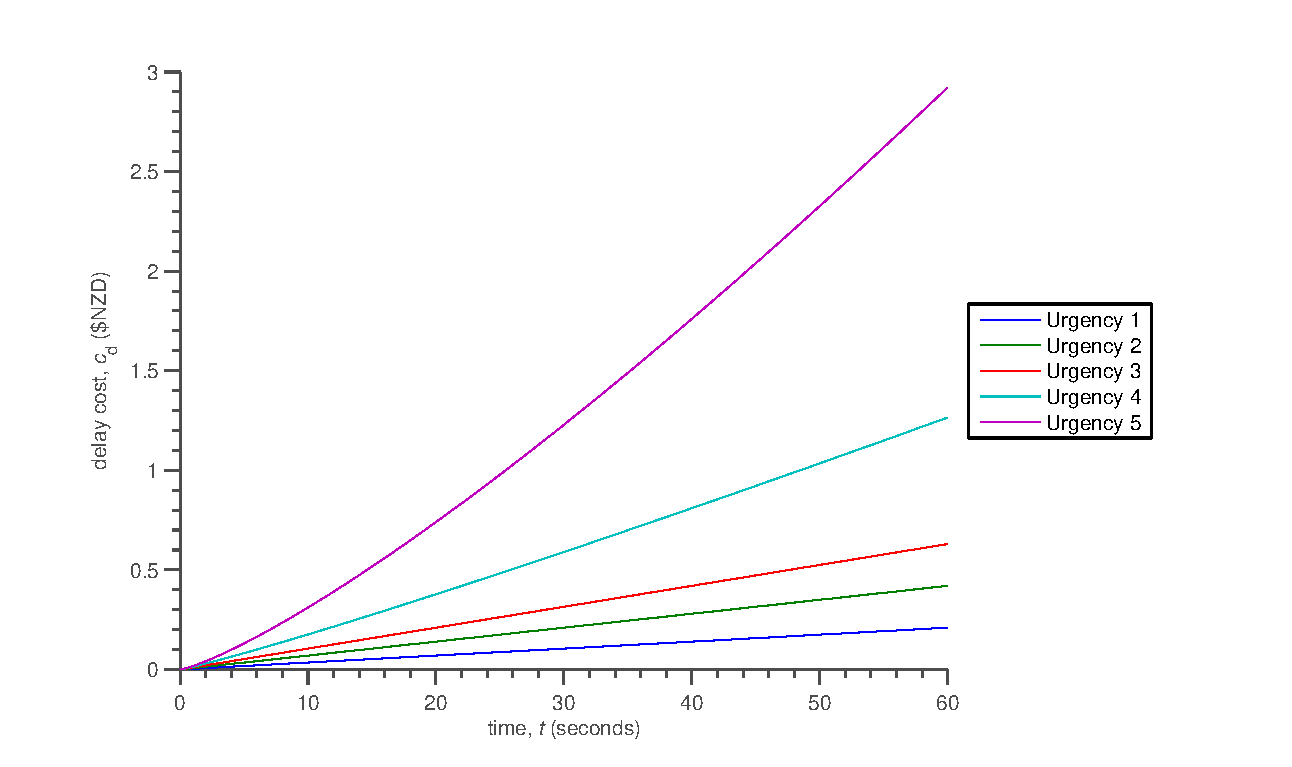
\includegraphics[scale=0.65]{delay_cost_per_urgency.eps}
	\caption{Cost of delay per time for a range of occupant urgency values, from time of zero seconds up to sixty seconds. }
\label{delaycosturgency}
\end{figure}

\section{PBTC System Design}

% the PBTC controller seeks to improve on existing delay or saturation based method by including the costs of travel for each vehicle in the control algorithm decision
 \citeasnoun{kesting2013traffic} describes the `Golden Rule of Traffic Flow Optimisation` as trying to homogenise traffic flow with respect to time, spatial arrangement, and local speed differences.

\subsection{Assumptions}

Design of a system for producing an optimal, minimal cost solution to phase assignment at any arbitrary controlled intersection is a difficult problem and evaluating such a system requires a sophisticated simulator capable of realistically modeling real world intersection geometrics, driver behaviours, and traffic flows. Development of these capabilities for simulation is an effort beyond the scope of this project. For this reason, the following assumptions have been made to simplify development of the PBTC control algorithm within this project:

\begin{itemize}
\item the control algorithm operates over a two-phase intersection, with each phase allocating green to one of two flows of traffic approaching the intersection only,
\item approaching vehicles represent straight through demand for the intersection only, no left/right split phases (i.e "arrow lights") are required,
\item the algorithm is limited to a single, isolated intersection only and does not consider any aspects of coordination between neighbouring intersection controllers.
\end{itemize}

\subsection{Vehicle-Controller Communication}

Communication between approaching or waiting vehicles and a PBTC controller at an intersection is required to provide inputs to the control algorithm to make a cost effective choice of phase timings based on the real-time traffic conditions. The implementation details of the required communication network is beyond the scope of this project and suggested as an area for future research. This project assumes that all of the necessary technology required for vehicles to send small packets of information to a controller exists in every vehicle using the road network, and each vehicle sends its own state information directly to the roadside intersection controller.

In the simulation developed as part of this project, vehicles approaching or waiting a PBTC controlled intersection broadcast their current state to the intersection controller every two seconds if the distance to the intersection stop line is less than 150 metres. There are two justifications for this behaviour, firstly; although in a simulated environment any object can feasibly read the properties of any other object at any time, it is important to consider the real world application of the system where network latency and limited network capacity are real problems that prevent instantaneous, real-time messaging with no delay. 

Secondly, consider a situation where a single vehicle is approaching a red light at an intersection where there is no demand for the competing green phase; in a stop-line actuated control system the vehicle will be forced to stop, wait at least six seconds for the lights to react and change phase, and then take off. By allowing a 150 metre broadcast window, a PBTC controller is able to respond to this situation and change the phase before the approaching vehicle has reached the lights, preventing them from stopping. The 150 metre window is based on assuming an approaching vehicle is traveling at a constant speed below 80km/h (approximately 22 m/s), requiring at least 133 metres of clearance given a typical controller requires 6 seconds of inter-green time to change a phase. In practice, it might be useful to be able to tweak the distance at which cars would be considered by the PBTC system based on the speed limit of the area. 

\begin{figure}[]
\centering
	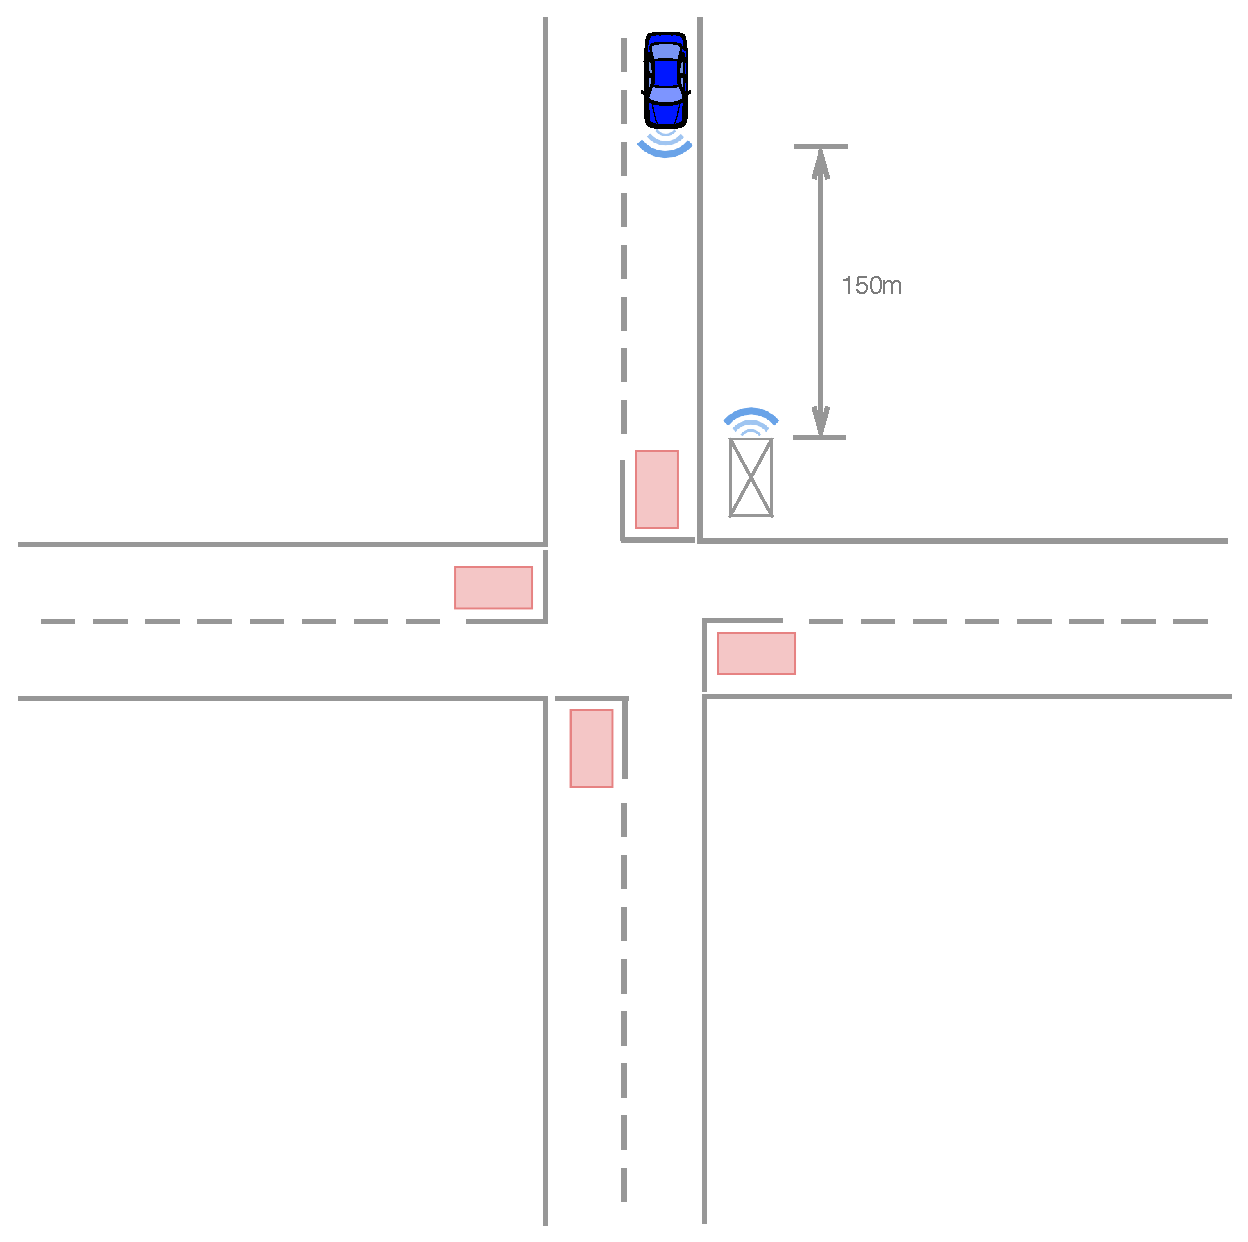
\includegraphics[scale=0.5]{intersection_diagram.eps}
	\caption{ Plan elevation of a simple four way intersection showing an approaching vehicle communicating with a PBTC controller. The distance of initial communication is shown as 150 metres. The position of stop-line detectors typically used by SCATS systems are shown in red. The PBTC controller is able to adapt to vehicle actuations in advance of the vehicle arrival at the stop line. }
\label{intersectiondiagram}
\end{figure}

\subsection {Control Algorithm Design}
\label{sec:PBTCDesign}

The PBTC control algorithm is a primary component of the PBTC system, designed to be executed by a roadside traffic controller to determine which phases should operate, the order of operation, and duration of each phase; in real-time. The primary objective of the PBTC control algorithm is to reduce the total economic cost incurred by vehicle movements  at PBTC controlled intersection, using traffic composition information communicated to a controller by vehicles in the network. 

Phases of an intersection are preconfigured based upon the geometry of the intersection. Each phase within the PBTC system contains an allocation of green or red signals to each light at a controlled intersection, such that no two competing traffic flows receive a green light at the same time in a phase. Two traffic flows are said to be competing if a collision would occur if vehicles on each flow entered the intersection at the same time. Each phase also defines a minimum time the phase must run for.  The minimum time condition is a safety consideration of the system, designed to allow enough time for at least one vehicle to pass safely through the intersection before the phase is changed. 

The order and duration of phases at a PBTC controlled intersection is determined by calculating aggregate costs of delay and operation for each approach of an intersection. A PBTC controller maintains a list of messages received from approaching or delayed vehicles that are used for calculation of the delay costs and operational stopping costs for each vehicle and aggregated to find the total costs for an approach. 

% primary cost of changing phase is the operational cost of stopping and delaying free flowing traffic
The primary cost of changing phases at a controlled intersection is the cost of stopping and delaying free flowing traffic. As a result, the standard operation for a PBTC controlled intersection is to run a set phase continuously until a phase change is determined to be cost effective and scheduled by the PBTC control algorithm. This behaviour is designed to produce minimal changes to the system, effectively maximising the homogeneity of free flowing traffic until the cost of interfering becomes low relative to the cost of doing nothing. 

A phase change is scheduled by a PBTC controller if the sum of the cost of stopping the traffic flow currently approaching a green signal, defined as the phase change cost or $c_\text{pc}$, is less than the total incurred cost of delay for all vehicles queued and waiting at any approaches displaying a red signal, defined as the phase delay cost or $c_\text{pd}$. The cost of stopping the traffic flow on a green signal also includes an estimation of the potential delay cost for each vehicle assuming they must be delayed \emph{at least} as long as the minimum condition for the newly scheduled phase. Equations X and X define the phase change cost and phase delay cost in a mathematical notation. 

\begin{equation}
	c_\text{pc} &= \sum_{v \in approaches.green.vehicles} c_\text{stop} + c_\text{delay(min)}
	\label{phaseChangeCostEq}
\end{equation}

\begin{equation}
	c_\text{pd} &= \sum_{approach \in approaches.red} \sum_{v \in approach.vehicles} c_\text{stop} + c_\text{delay(min)}
	\label{phaseDelayCostEq}
\end{equation}

If this condition is true at any time, the algorithm enters a phase change sequence. During a phase change sequence, a lookahead heuristic is applied to find the minimum potential cost incurred as a result of the change. Based on a predefined lookahead table size, the controller estimates the total cost of changing phase for each second from zero up to the table size, constructing a table with each row representing a time in seconds and the cost of stopping the phase at that time. The controller then dynamically extends the current phase duration by the number of seconds that corresponds with the lowest cost value in the lookahead table.

The lookahead method used in the PBTC control algorithm is an optimisation method performing a local search for a time of changing phases that incurs the least cost to the system. For example, consider an intersection where two vehicles have been waiting at a red signal for 60 seconds, and the cost of delay has exceeded the cost of stopping the opposing traffic flow receiving a green signal. If two vehicles are approaching the intersection on the freely flowing approach but are close enough to stop if the phase is changed immediately, the cost of the change includes the operational cost of stopping the two vehicles and the cost of delaying the vehicles for the minimum duration of the next phase. 

Due to their distance from the intersection and current velocity, after one additional second the two moving vehicles may pass through the intersection and these costs are avoided, with the trade-off cost being one more second of delay for the two waiting vehicles. Unless the two waiting vehicles have high urgency and a high number of passengers, the cost of an additional second of delay is likely to be marginal. The lookahead procedure of the PBTC control algorithm will evaluate the total cost of extending the current phase by a fixed number of seconds to allow the moving vehicles to pass, and extend the current phase by the calculated minimum time if it is found to be less than the cost of an immediate change.

\begin{algorithm}[H]
 \SetAlgoLined
 \KwData{
 	c_p: current phase, n_p: next scheduled phase, a: set of approaches, K: lookahead window size
 }
 \KwResult{ minimal cost time until phase should be change executed }
 \Begin{
  set $totalStoppingCost$ = 0 \; \\
  set $totalDelayCost$ = 0 \; \\
  \For{approach in approaches}{
  	\If{approach signal is red} {
		add cost of delay for all vehicles queued on approach to $totalDelayCost$ \;
	} 
	\Else{
		add cost of stopping and cost of minimum delay for all vehicles on approach to $totalStoppingCost$ \;
	}
  }
  \If {$stoppingCost < delayCost$} {
  	set lookaheadTable = [] \;
	\For{$i := 0$ to K} {
		lookaheadTable[i] = cost of delay for all stopped approaches over $i$ + cost of stopping for all vehicles that cannot clear the intersection after $i$ seconds \;
	}

  set extendedGreenTime = index of minimum value in lookaheadTable \;	
  return extendedGreenTime \;
}
return -1 \;	 \tcc*[r]{no change scheduled}
 }
 \caption{PBTC phase scheduling algorithm}
\end{algorithm}

% discuss lookahead search tree from other paper here

\section{Evaluation Methodology}

Performance evaluation and analysis is required to determine the effectiveness and appropriateness of the PBTC system. Performance evaluation of traffic control methodology is made difficult by the proprietary and commercial nature of traffic control algorithms and the software systems that implement them. All New Zealand intersections are controlled by the SCATS system, which is commercially developed in Australia and in use in many countries worldwide. No test bed or performance evaluation software is available for SCATS, and as a result a direct comparison with the SCATS implementation is not possible.

An alternative to a direct comparison with the SCATS system considered during the development of this project was to develop a simplified and approximate system that was based off the methodology of SCATS. While this method had the advantage of being able to produce a flexible estimation system that can be easily benchmarked against the PBTC system, there are disadvantages related to implementing an approximation to be representative of the real system. 

Firstly, there is a very limited amount of publicly accessible information related to the design and implementation of the SCATS control algorithms. One of the very few papers available described some algorithms of the very first version of the SCATS system \citeasnoun{lowrie1982scats}, however it is not easy to know how much the system has improved since this paper was published. Secondly, it is not easy to determine how good of an approximation any simplified implementation of SCATS would be without being able to benchmark against the real system leading to potentially inaccurate comparisons. 

As a result of these two limitations of developing a custom, simplified SCATS implementation, the evaluation component of this project was designed based on using reports generated by SCATS containing phase times and traffic conditions of the SCATS system operating on intersections in Wellington over a 12 hour period. The reports used during evaluation were generously provided by the Wellington City Council (WCC), who operate SCATS for all of the intersections in the central Wellington City area. 

SCATS allows WCC engineers to produce reports showing data and intersection state information for every cycle of operation, including exact phase times and the number of vehicle detections per phase. The evaluation component of this project was designed to use the information contained within these reports to reconstruct a realistic representation of SCATS operation in Wellington. This method was preferred over the custom implementation of SCATS because of the relative ease of generating vehicle arrivals and scheduling phase times based off the SCATS reports in simulation. As a result, this method of evaluation the closest to an accurate representation of the real SCATS behaviour, and is easily evaluated over an extended period of operation. 

The 12 hour period of operation was determined with consideration to the typical profile of traffic in the central Wellington City area during a day. A typical day for an inner city intersection is characterised by two "peaks" of traffic congestion in the morning and evening for around 1-2 hours each. Traffic composition around these peaks typically consists of motorists on a morning or evening commute to and from inner city offices for work. By evaluating traffic performance over a 12 hour period from 7AM to 7PM, these peaks can be included in the evaluation, creating a range of traffic conditions for performance analysis. 

%The primary goal of the PBTC system is to reduce the economic costs of delay at a controlled intersection and as a result, evaluation metrics discussed here are designed to measure the impacted costs of running the system over an extended period of time for an intersection.








\chapter{Simulator Design and Implementation}

The following chapter describes the design and implementation of PBTSim, a software package to allow for simulation and evaluation of priority based traffic control. To produce a representative comparison with existing SCATS-based systems, creating a realistic simulation environment was a key implementation challenge, and a primary objective of this project. The outcomes discussed in this chapter are:

\begin{itemize}
\item using the open-source software package MovSim as a framework for implementation of PBTSim,
\item implementing a simulation scenario for development and evaluation,
\item extending the Movsim package within PBTSim to support development of the PBTC control algorithm and allowing for future control algorithms to be added easily,
\item development of a parser for SCATS log files, to allow for traffic flow rates and traffic signal phase timings to be read from a SCATS log file and used in simulation,
\end{itemize}

\section{Simulation Platform}

A primary challenge of measuring and evaluating performance of an adaptive traffic control system is the requirement to simulate realistic traffic conditions with sufficiently measurable results. Software for simulating traffic control methods is typically developed by vendors of a particular system and as such is proprietary and not available for research. Because of this, an open-source tool called Movsim has been used as a framework for development and evaluation within this project. 

Movsim (Multi-model Open-source Vehicular-traffic Simulator) is an open-source, Java-based traffic simulator implementing multiple time-continuous, car-following traffic models designed for investigating traffic dynamics; currently under active development. Movsim is based upon the work of \citeasnoun{kesting2013traffic} and implements a wide range of configurable vehicle-following, acceleration, and lane changing models that determine individual vehicle movement within the simulation.

\begin{figure}[]
\centering
	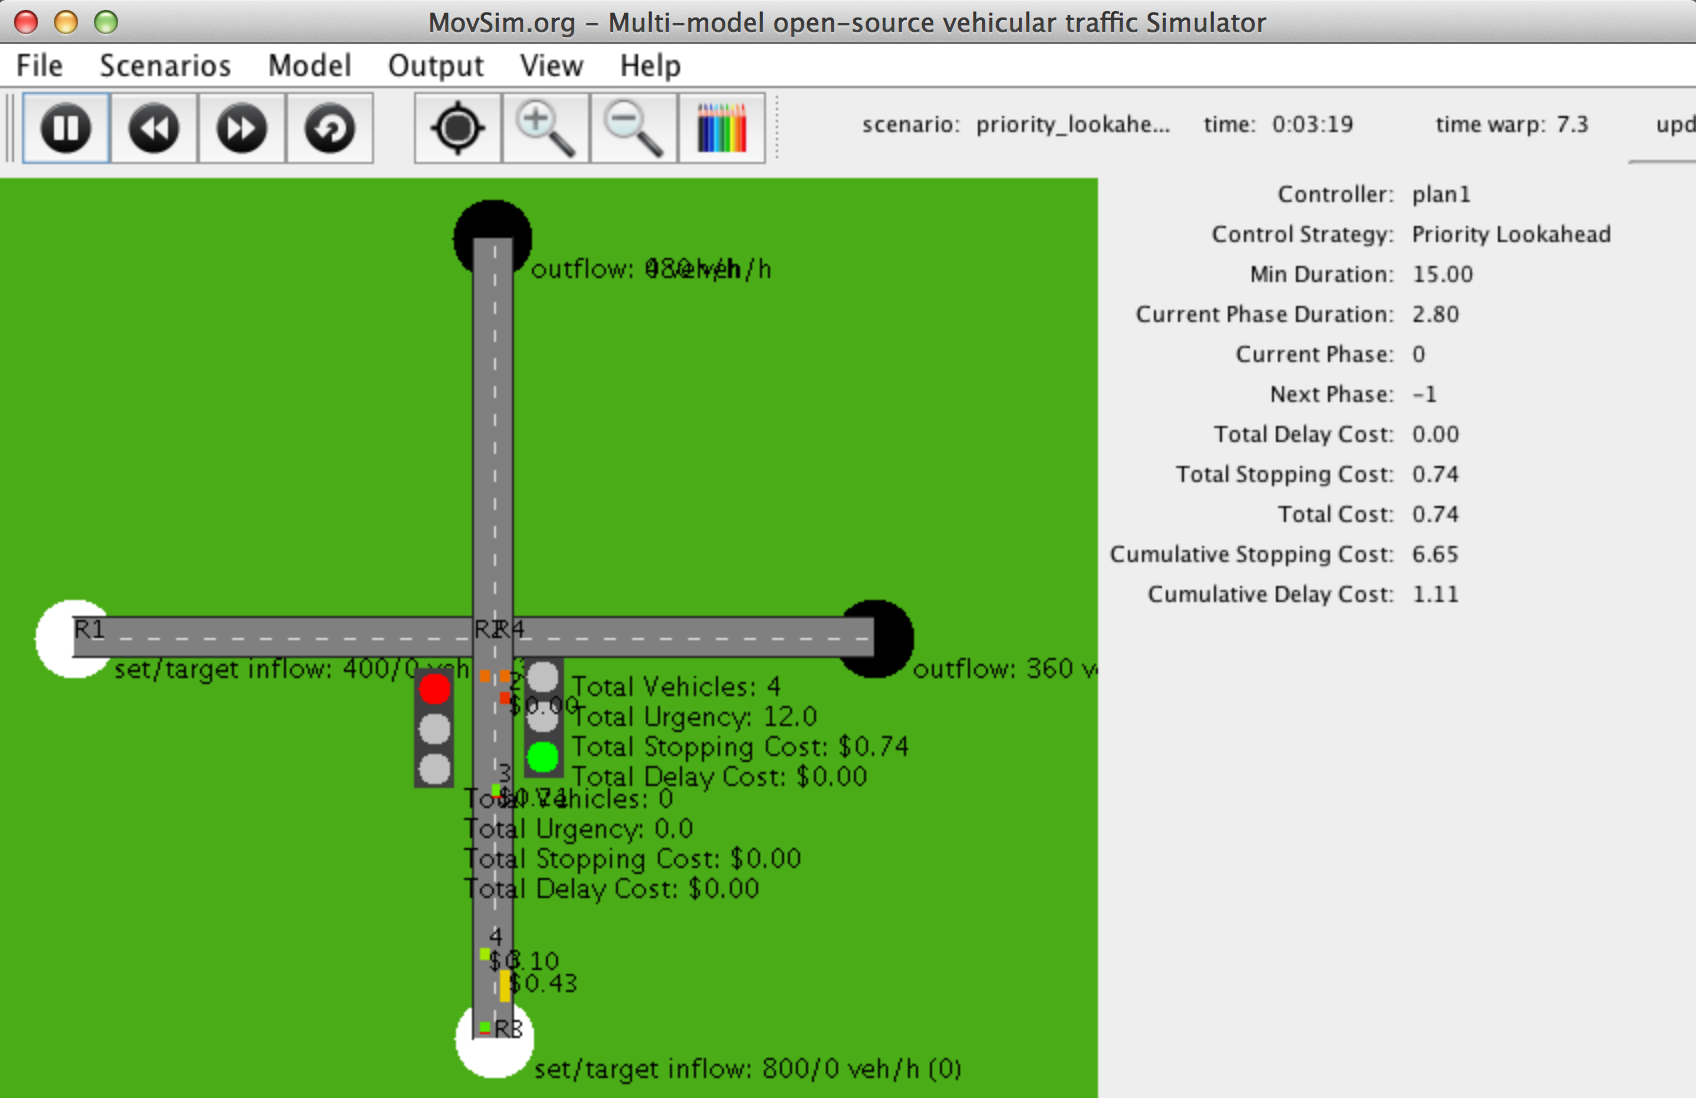
\includegraphics[scale=0.35]{movsim-interface.png}
	\caption{ A screenshot of the MovSim Graphical User Interface running a simulation of the four-way intersection scenario used during design and evaluation of the PBTC control system. }
\label{intersectiondiagram}
\end{figure}

All software artefacts produced during this project were implemented within a fork of the Movsim project, which we have named PBTSim (Priority Based Traffic Simulator). PBTSim is a software application that allows for simulation and evaluation of traffic control methods based on the vehicle priority model described in Chapter 4. While priority based traffic model features specific to this project are maintained in PBTSim, general purpose features and improvements to the Movsim project have been offered back to the original Movsim repository for consideration of the maintaining authors.

Limitations of using the MovSim project as a base simulation tool for the PBTSim include lack of support for bi-directional traffic flow and turning behaviour at intersections, both requirements for accurate modeling of a real world road network. Both of these features are areas of future development for the MovSim project. The sophisticated traffic modeling capabilities of the MovSim application, have outweighed these limitations during development of the PBTC system.

\section{Scenario Design}
\label{sec:ScenarioDesign}

The MovSim simulator is designed to be highly configurable and uses XML files as specifications for the simulations that will be executed. One of the two road network description files required by MovSim is an OpenDrive network specification file which defines the geometry, order, and connections between roads which are structured in XML. OpenDrive is an "open file format for the logical description of road networks" \cite{opendrive}. The format is extremely descriptive and supports a large number of geometric constructs to generate realistic road networks. As MovSim required the use of OpenDrive, no alternative road network description formats are discussed here.

The intersection configuration designed and implemented for evaluation purposes within this project consists of two one-way approaches, each with two vehicle lanes and was based on availability of data for real-world intersections in Wellington City. As this two-way intersection configuration is a common design, the configuration files were submitted back to the Movsim repository as an example, and accepted by the Movsim authors. 

% include snippet example in appendix?

Although OpenDrive supports a large number of realistic road network configurations, the implementation supported within the MovSim simulator is limited to a subset of these. Currently, MovSim has no support for bi-directional roads in OpenDrive; although this feature has been under active development by the MovSim authors for a number of months. Without bidirectional roading, the intersection configuration in this project has been limited to two-phase "crossroads" intersections with two approaches of one-way traffic, such as above, only. 

\section{Phase Model}

Movsim allows for customisable phases to be configured in the project description file, an XML document describing user-defined settings for traffic composition, simulation variables, and traffic controller plans. Traffic controller phases can be defined in the project description file as an ordered list, with each phase including a list of the state (green, amber, or red) for each traffic light for a given controller. 

\begin{figure}[]
\centering
	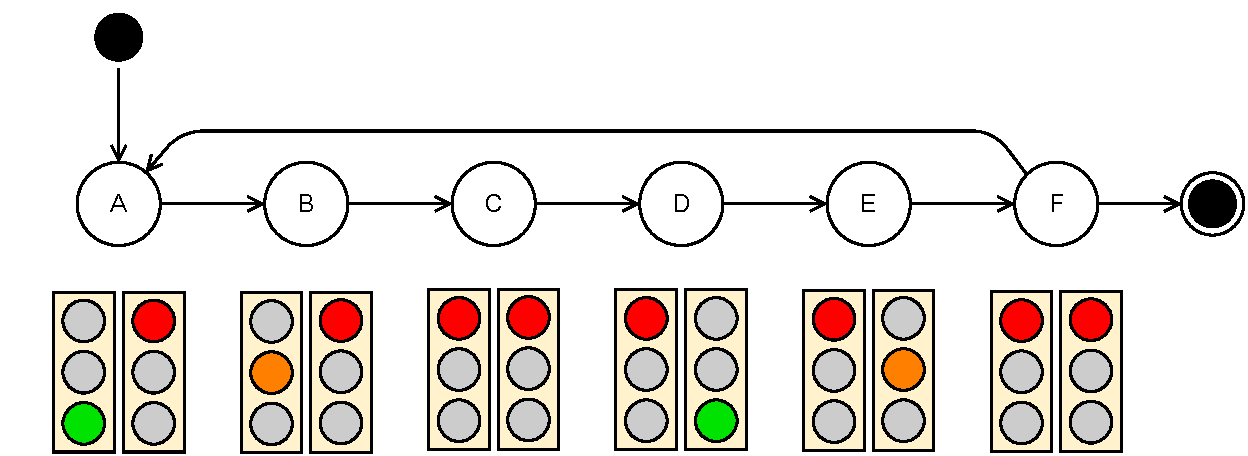
\includegraphics[scale=0.60]{movsim-phases.pdf}
	\caption{ A diagram of the available phase states and transitions of a "two-phase" configuration within the Movsim simulator. Movsim requires intergreen and all-red periods to be configured as individual phases and does not allow a simple mechanism for skipping, repeating, or alternating the order of configured phases. }
\label{movsimphasediagram}
\end{figure}

The phase model used in most modern traffic control systems is a finite state machine consisting of a set of states for each traffic light connected to the controller, with a set of constraints that define valid states and allowed transitions between states. The basic phase model implemented within the Movsim project implements this model, however Movsim requires a distinct phase for each period of intergreen time. For example, Figure ~\ref{movsimphasediagram} shows how a traditional "two phase" intersection requires a minimum of six configured phases to incorporate intergreen and all-red periods of operation using the Movsim model. This model requires more design and configuration effort, and does not enforce intergreen periods of operation between two active phases.

To solve this problem, a new phase model was developed for the PBTSim simulator during this project. The developed model is similar to the phase model used by SCATS, where each phase includes a fixed number of seconds as minimum time, maximum time, and intergreen time. It is assumed that during an intergreen period any traffic lights currently displaying a green signal transition to yellow, and all others remain the same. Using this model, the need for additional phases to explicitly define intergreen periods of operation is redundant and the PBTSim simulator enforces intergreen constraints between active phases. Figure ~\ref{PBTSimphasediagram} shows a state diagram of the PBTSim representation of the same "two phase" configuration described in Figure ~\ref{movsimphasediagram}.

\begin{figure}[]
\centering
	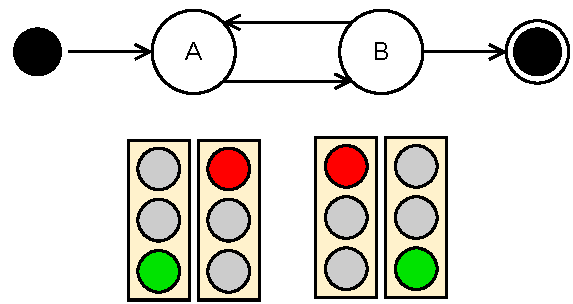
\includegraphics[scale=0.60]{pbtsim-phases.pdf}
	\caption{ A diagram of the available phase states and transitions of a "two-phase" configuration within the PBTSim simulator. Integreen and all-red times are encoded as properties of each phase and the scheduling of these phases is moved to application logic to simplify the phase configuration. }
\label{movsimphasediagram}
\end{figure}

%2
While appropriate for simple examples and fixed-time phases, the basic Movsim implementation of phase configuration is not appropriate for advanced controller strategies, including the PBTC strategy, where skipping phases with no traffic demand is desirable. It is difficult to express skipping of phases in the Movsim phase model, as there is no clear distinction between an intergreen phase and an "active" phase to indicate which phases are allowed to be skipped. For example, skipping the "next" phase will cause the traffic controller to skip the intergreen phase and change to another active phase, rather than the desired behaviour of skipping the next active phase.

The new phase model of PBTSim addresses this problem as integreen and all-red periods of operation are enforced during transitions between active phases, rather than phases themselves. As a result, expressing skipped phases or operating phases out of order is greatly simplified. 

The new phase model developed during this project has been provided to the Movsim authors as a potential general purpose improvement.

% good up to here jm 04.10.13

\section{Vehicle Priority Simulation}

Priority based traffic modeling is a concept specific to this project and is not implemented in any form within the Movsim simulator. To allow for implementation of the PBTC control system, PBTSim implements the priority model described in Chapter 4 for all vehicles, and simulates communication between vehicles and a traffic light controller as required by the PBTC control system.

\subsection{Traffic Composition}

The priority model described in Chapter 4 assumes that occupants of all vehicles on a road network have an urgency of travel, defined as a discrete integer between one and five. As this is an arbitrary, relative scale of motorist urgency, statistics of the distribution of driver urgencies for a given time or particular intersection are unknown and not easily measured.

As a result, the distribution of urgency values of traffic within the PBTSim system is estimated using an enumerated probability distribution which assigns an arbitrary probability of occurrence to each urgency value for each class of vehicle within the simulation. Table ~\ref{urgencydistribution} shows the probability distribution of urgency values for each class of vehicle in the PBTSim system. The distributions of urgency values are relatively weighted to indicate reasonable assumptions on vehicle urgency, which are difficult to empirically measure and it is beyond the scope of this project to do so, e.g. by surveying characteristics of vehicles and road users at an intersection. 

\begin{table}[]
\begin{center}
\begin{tabular}{lrrrrr}
\toprule
 & \multicolumn{5}{c}{Passenger Urgency} \\
 \cmidrule(lr){2-6}
Vehicle Class & 1 & 2 & 3 & 4 & 5 \\
\midrule
Car (Light Vehicle) & 0.2 & 0.25 & 0.395 & 0.15 & 0.005  \\
Bus (Heavy Vehicle) & 0.3 & 0.5 & 0.2 & 0.0 & 0.0 \\
Truck (Heavy Vehicle) & 0.1 & 0.5 & 0.3 & 0.1 & 0.0 \\
\bottomrule
\end{tabular}
\end{center}
\caption{Probability values for an enumerated integer distribution of individual vehicle urgencies. Each urgency value in the range 1--5 is associated with a probability of occurrence for a single vehicle. }
	\label{urgencydistribution}
\end{table}

Probability values are assigned to give a one-sided distribution that assumes there are lower proportions of truly urgent road users than not. Buses and trucks have relatively lower average urgency values compared to passenger cars. This measure is used to reflect that public transport is by its nature unreliable for each single passenger, hence most passengers using public transport allow more time than required to reach their destination and that the majority of freight trucks operate on long inter-city journeys, hence the proportion of time potentially spent waiting in traffic lights in a city is small compared to the relatively long journey time.

\subsection{Approach Communication}

A requirement of the design of the PBTC control system is that all vehicles approaching an intersection must broadcast their position, physical properties, and required passenger characteristics to a traffic controller. As Movsim was not designed with this requirement in mind, a new system of simulated communication between vehicles and traffic controllers had to be designed for the PBTSim simulator.

Each traffic controller within the simulation maintains a list of broadcasts they have received as a map and each new broadcast replaces any existing broadcast from each unique vehicle. An individual broadcast contains properties required by a controller in order to calculate operational stopping cost and delay cost estimated for each individual vehicle, specifically vehicle weight, speed, acceleration, urgency, number of passengers, and distance to the intersection stop-line. Once a vehicle has cleared the stop-line of an intersection, their broadcast is removed from the traffic controller map.

In order to ensure that the PBTSim environment is representative of a realistic road network and network infrastructure, efforts are made to ensure that the simulated communication between approaching vehicles and a traffic controller includes consideration of the challenges of a real-world communications network. In a simulated environment, vehicle properties can be broadcast instantly, without network costs or delay; however, in reality network topology and bandwidth limitations are factors that reduce the availability of broadcasts. To introduce consideration of networking latency into PBTSim, a two-second delay is imposed on each broadcast from an individual vehicle. This is not designed to be an accurate representation of network imperfections, but does reflect consideration of these factors.

An alternative design considered involved allowing delay and stopping costs to be calculated and broadcast by the vehicle itself. This method has the advantage of reducing the amount of calculations that are required to be made by a traffic controller, however this distributed computation is more difficult to implement successfully and there are no guarantees that all vehicles will implement the same cost calculations. This method is also difficult to update if changes to the cost calculations were desired after installation.

\section{Control Strategies}

Movsim includes a basic implementation of traffic control capable of operating an ordered list of traffic light phases defined in the simulation configuration file, however the implementation is limited to fixed-time phase control only, where each phase runs for a predetermined number of seconds before transitioning to the next phase. In order to allow for evaluation of multiple phase control strategies to be tested during simulation, a more sophisticated architecture design was implemented during development of the PBTSim system. 

Changes made to the traffic control architecture of PBTSim during this project are designed to be modular and avoid limiting the scope of future work or potential for implementation changes. Figure ~\ref{controllerclassdiagram} shows a UML class diagram of the type relationships in the traffic control architecture of PBTSim. ControlStrategy is a Java interface class added to PBTSim which implements the Strategy Pattern, an object-oriented design pattern that allows for dynamic selection of a strategy implementation at runtime. This pattern is well-suited to the design of the control strategy algorithm as new strategies (such as the PBTC system) can be added to the system by implementing the strategy interface and defining their own behaviour. % cite strategy pattern here

The ControlStrategy interface is called by a TrafficLightControlGroup class, which controls the state of lights within the simulator. Methods of the ControlStrategy interface allow a TrafficLightControlGroup to check if conditions for scheduling a phase change have been met and acknowledge the change once it has been made. Each concrete implementation of the ControlStrategy class can implement their own conditions and strategies that will trigger a change. This relationship creates a separation of concerns between controlling traffic light state and defining traffic light behaviour, allowing for new behaviours to be easily added independently of all other existing strategies. 

\begin{figure}[]
\centering
	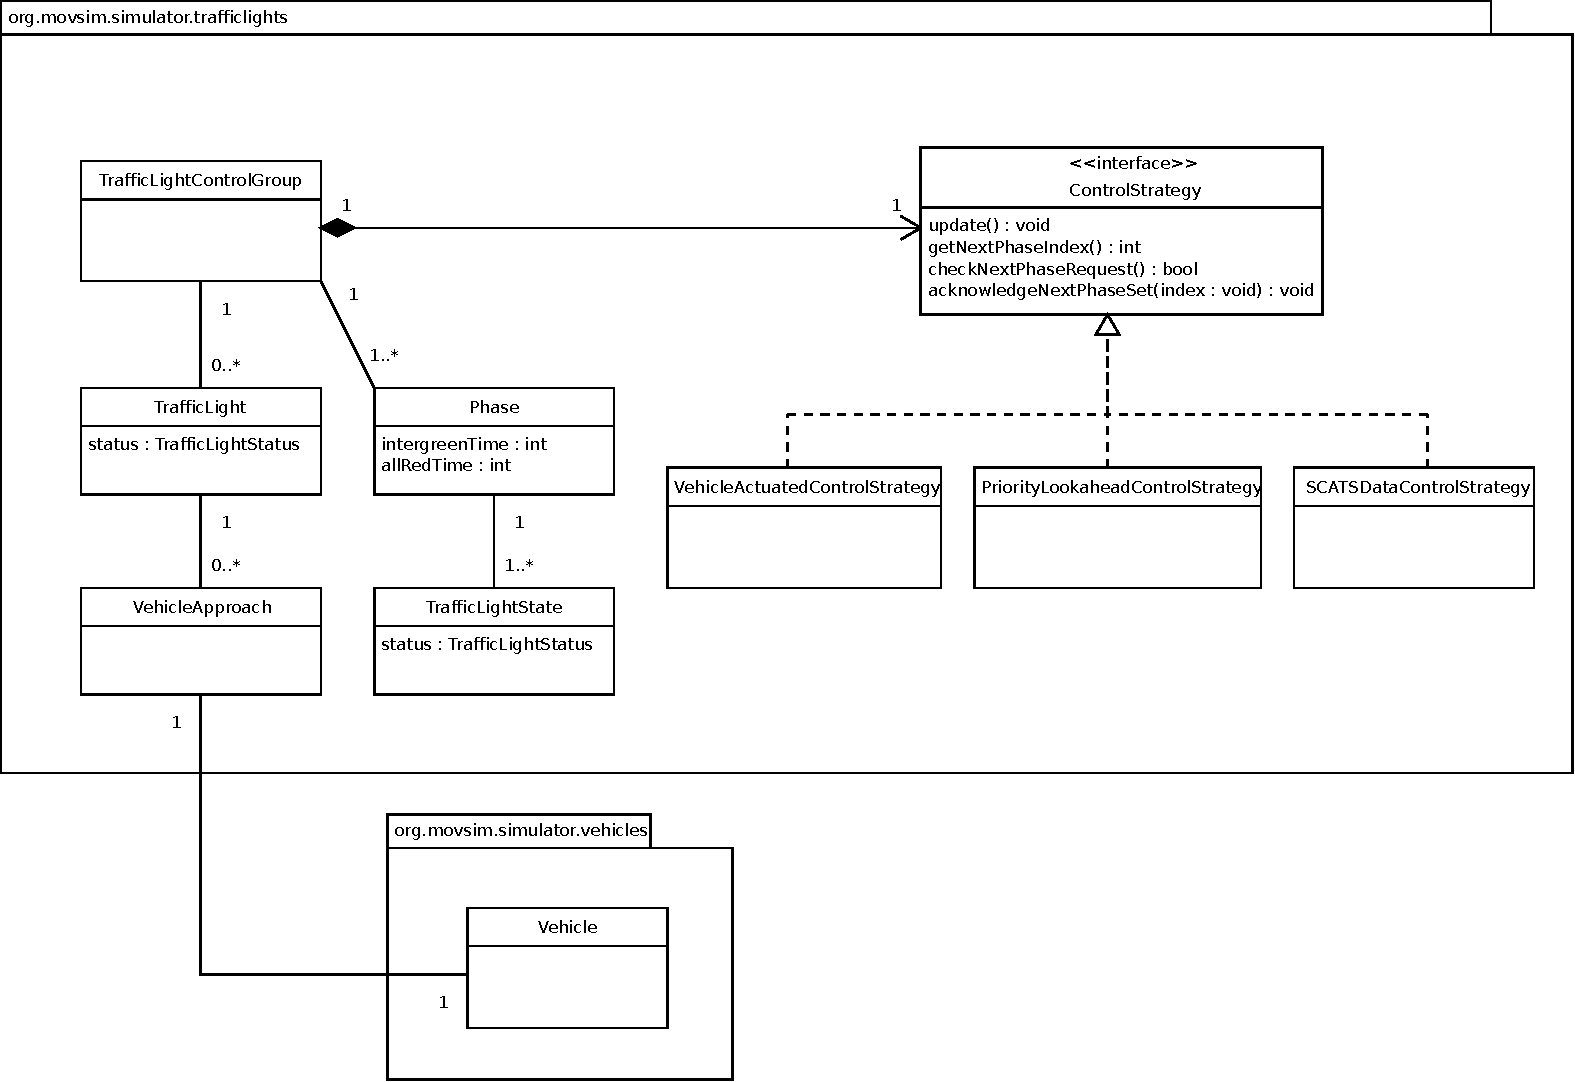
\includegraphics[scale=0.60]{controller_class_diagram.pdf}
	\caption{ A UML class diagram showing the use of the strategy pattern between the TrafficLightControlGroup and ControlStrategy types. ControlStrategy is an interface defining methods required by the TrafficLightControlGroup to change the phase of a set of traffic lights. Three strategies implementing the ControlStrategy interface are shown. Each concrete strategy implementation has a different internal set of conditions to trigger phase changes. }
\label{controllerclassdiagram}
\end{figure}

% good up to here

\section{Implementation of the PBTC Control Strategy}

The PBTC control algorithm described in Section ~\ref{sec:PBTCDesign} is implemented as a concrete ControlStrategy implementation within PBTSim. The strategy implementation of the PBTC control algorithm consists of two primary phases of operation; approach cost calculation and phase scheduling. 

The PBTC control algorithm implementation dynamically calculates the sum of the individual estimated delay and operational stopping costs for all of the vehicles on each approaching link of the intersection at each simulator update. 
The current phase of a PBTC traffic controller operates continuously until the calculated cost of delay on all stopped approaches exceeds than the cost of stopping green approaches, at which point the next phase is allocated and the controller enters the phase change sequence. Once the controller has entered the phase change sequence, it is  committed to changing phases and the lookahead optimisation method is employed to determine whether the phase should change now, or some point in the future, based on the real-time position and state information of vehicles on approaching links. 

% this section is good
\subsection{Lookahead Optimisation}

PBTSim implements the PBTC control algorithm's lookahead features using a map to construct a table of cost values a the end of each phase, once the phase change sequence has been initiated. The lookahead table includes an estimate of the instantaneous change costs for all vehicles known to the PBTC controller at the time the phase change sequence was entered. For each second up to the defined size of the lookahead table, $K$, the PBTC control strategy estimates the cost of changing phases by finding the sum of the cost of stopping, and the cost of delay at least equal to the minimum duration of the next phase in the controller sequence for every individual vehicle approaching a green signal, and the sum of the cost of stopping and cost of delay for the duration of the current lookahead for any vehicles approaching or queued at a red signal. 

To estimate the costs of a phase change each second up to the lookahead time, a PBTC system needs to identify if each vehicle approaching a light currently displaying a green signal will be stopped by the phase change and hence incur the cost of stopping, or will clear the intersection within the number of seconds the change will be scheduled for and have no additional costs incurred. In a free-flowing traffic situation, the distance traveled by a vehicle in a fixed time frame can be estimated using the vehicles speed and acceleration only. For example, if a PBTC controller is considering a phase change for an intersection 5 seconds from the present time, and a vehicle is approaching at 10m/s at a distance of 30 metres, the vehicle will have passed over the intersection stop line within 3 seconds therefore will not be affected by the phase change.  However, in congested traffic where vehicles are queued, whether or not a given vehicle, $v$ in the queue will clear an intersection within $t$ seconds is dependant on the speed and acceleration profiles of vehicles in front of $v$, and as a result is significantly affected by driver behaviours and instantaneous traffic conditions. 

Developing and implementing such a model for simulation and evaluation of the PBTC system is an effort beyond the scope of this project and as a result, empirical measurement of clearance times and distances within PBTSim was conducted to estimate the worst-case conditions of congested traffic and identify the maximum distance a vehicle could be from a traffic light to clear within a fixed range of seconds. The experiment was run by operating a green phase for a fixed number of seconds at an intersection with a volume of traffic exceeding the capacity of the network, to generate a queue. The distance of the furtherest vehicle from the intersection at the time that the phase began that cleared the intersection within the time frame is the result, repeated a number of times to find a maximum. 

Measurement results were used to create a map of key-value pairs consisting of the time in seconds, and the maximum distance from a traffic light a vehicle could expect to clear the intersection within the time frame. Table ~\ref{vehiclecleardistances} shows the measured results used by PBTSim to determine whether each vehicle will clear a traffic light within a given timeframe. If a vehicle has a speed of less than 2.5m/s when approaching a traffic light, it is assumed to be in queue and the estimated clear time is determined from the table.

\begin{table}[]
\begin{center}
\begin{tabular}{rr}
\toprule
Phase Duration ($s$) & Queue Clear Distance ($m$) \\
\midrule
10 & 22.12 \\
15 & 40.03 \\
20 & 58.10 \\
25 & 80.15 \\
30 & 94.40 \\
35 & 111.47 \\
40 & 133.50 \\
\bottomrule
\end{tabular}
\end{center}
\caption{ Estimated maximum intersection clearance distances used by PBTSim to determine if a queued vehicle will pass an intersection before the end of a phase. The time is given as the duration of green time remaining in the phase, and the distance is the maximum expected distance a vehicle can be queued from the intersection stop-line to clear within the allowed time. }
\label{vehiclecleardistances}
\end{table}

\section{Implementation of a SCATS Control Strategy}

% can use the SCATS data to determine arrivals and signal settings each cyclex
Development of a SCATS representation is a requirement of the evaluation process of this project. As SCATS is deployed on most of the controlled intersections within New Zealand and uses an adaptive traffic control algorithm to respond to near real-time traffic demand, it is appropriate for comparison with the PBTC control algorithm.

As SCATS is a commercial system, no software or algorithms are available for public research. As a result, the SCATS implementation developed for PBTSim is designed to recreate a realistic representation of real-world SCATS behaviour using an available log file of vehicle arrivals and allocated phase times at different intersections in Wellington City. An example of the SCATS log file format is shown in Appendix A. Log files for intersections in Wellington City were provided for a 12 hour period of a typical day by the Wellington City Council.

Each SCATS log file consists of an ordered sequence of data blocks for each single cycle of operation of a given traffic light controller, sent to SCATS by the controller at the end of each cycle. The cycle block contains state information required by SCATS to calculate the phase timings for the next cycle, including number of vehicle detector actuations per approach, i.e. the number of vehicles that entered the intersection on each approach; and the order and time of each of the phase splits run by the controller during that cycle. 

The design and implementation of a software package to simulate SCATS behaviour involved replicating the arrivals recorded by SCATS over the fixed period of the log, and developing a control strategy to operate phase times for each cycle of the log. Figure ~\ref{scatsclassdiagram} shows a class diagram overview of classes in PBTSim designed to add SCATS simulation capabilities. 

% good up to here
\subsection{Vehicle Arrivals}

The number of vehicles arriving or waiting at an intersection, also referred to as the saturation or flow rate of an intersection, is an independent variable determined by the number of vehicles on the road, criticality of an intersection to a road network. When comparing the performance of multiple traffic control strategies, the flow of vehicles input into the system should remain constant between each experiment. To account for this in the evaluation of the PBTC control system, SCATS log files are used to determine the flow rate of vehicle arrivals in PBTSim. 

SCATS provides the number of vehicle actuations recorded by each stop line inductive loop detector, for each cycle contained within an intersection log file. As SCATS detectors are placed on the stop line of each approach at an intersection, it is assumed that the number of vehicle actuations at each detector is approximately equal to the number of vehicles that passed through the intersection during a given green phase and the number of vehicles that arrived on that approach over the entire cycle. By using the cycle duration as a range for estimating the exact arrival time of a given vehicle approaching an intersection, it is possible to introduce a probability function that allows for a proportion of vehicles to arrive early during a red phase, and the remainder to arrive on time during the green phase of a particular traffic light. As no other information related to the time of vehicle arrivals is available, arrival events are implemented using a Poisson arrival process. 

During a PBTSim simulation, the Poisson process is used to generate an estimated time to the next arrival after each simulated arrival has taken place. The Poisson arrivals implementation is a general purpose improvement over the linear arrivals model that was previously implemented in Movsim has been submitted back to the original Movsim repository as a configurable option to benefit other research.

These assumptions provide a reasonable estimate of the arrival time of vehicles to each queue at an intersection, as it is not possible to know the exact time of arrival and waiting time for each vehicle using only SCATS log files. The consequence of these assumptions is that generated arrival times may not be representative of the arrival times that occurred during the real-world scenario that the SCATS log files reflect, although on average it is expected the simulated arrival times will be close approximations of real-world arrivals. 

\subsection{SCATS Control Stategy}

The SCATS representation developed for PBTSim is designed to implement the ControlStategy interface class to work seamlessly with the traffic lights and controller classes of PBTSim.

The SCATSDataControlStrategy is a Java class that dynamically operates the measured phase durations contained within a SCATS log file by requesting new data from the SCATSDataParser each cycle. The SCATSDataParser is a singleton class which waits for a prompt for data from a SCATSDataControlStrategy or TrafficSource instance. The parser reads a cycle block from the log file and returns a list of phases and their durations to the SCATSDataControlStrategy, and updates each TrafficSource with a new arrival flow rate based on the phase times and vehicle arrivals measured in current cycle being read from the SCATS log. The SCATSDataControlStrategy allocates phases in order based on the list returned from the data parser and continues until the list is empty, at which point it requests another cycle and so forth.

The SCATSDataParser class is designed to respond to requests for data as it does not implement its own update method so does not have a measure of simulation time elapsed. This method ensures that a new cycle is only read from the log after the previous cycle has ended. One disadvantage of this method is that individual timers kept by each TrafficSource are not synchronised so after the cycle duration has expired, each individual TrafficSource will attempt to request the data parser to read a new cycle. Multiple cycle reads are avoided by reseting each TrafficSource after the first one has called for an update.
























\chapter{evaluation}

\section{Methodology}

\subsection{Scenario Configuration}

\begin{figure}[]
\centering
	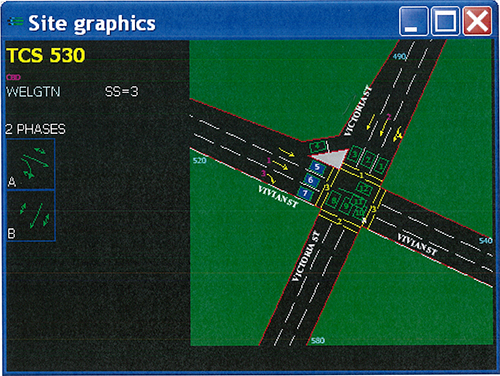
\includegraphics[scale=0.5]{scats-vivian-victoria.png}
	\caption{ The intersection of Vivian Street and Victoria Street in Te Aro, Wellington City, as viewed in the SCATS management application in use by Wellington City Council. }
\label{intersectiondiagram}
\end{figure}

%%%%%%%%%%%%%%%%%%%%%%%%%%%%%%%%%%%%%%%%%%%%%%%%%%%%%%%
\backmatter
%%%%%%%%%%%%%%%%%%%%%%%%%%%%%%%%%%%%%%%%%%%%%%%%%%%%%%%

%\bibliographystyle{ieeetr}
\bibliographystyle{harvard}

\bibliography{sample}

\begin{appendices}

\chapter{Terminology}
\label{appendix:terminology}

Traffic control engineering involves specific terminology to refer to different signal controls, timing plans, and controller types. This section offers a brief introduction of traffic signal control and terminology.

Modern intersections with traffic signals are controlled by a roadside \emph{signal controller}. An intersection consists of a number of \emph{approaches} which are distinct roads leading to a point of intersection. Controllers switch power to signal lanterns and determine the sequence of display for each set of lights, operating under the safety requirement that no two conflicting approaches receive green signals simultaneously. A typical controller operates lights in sequences called \emph{phases}, which are dynamic length allocations of green light time to a set of non-conflicting flows at an intersection. \cite{papa2003review}. Typically, modern controllers include the following fixed or dynamic time allocations within a phase:

\begin{itemize}
\item \emph{late start time}, a fixed length of time a green light may be delayed for safety of other movements (e.g. pedestrian protection)
\item \emph{minimum green time}, a fixed length of time that a phase must operate before changing
\item \emph{intergreen time}, a fixed length of time required to operate amber and red signals at the end of a phase, typically at least 6 seconds. 
\item \emph{extension green time}, a dynamic length of time allocated to a phase determined after all required fixed times have been deducted from the total phase tie. 
\item \emph{maximum green time}, if the addition of the previous four time allocations exceeds the fixed maximum green time the phase is forced to change. 
\end{itemize}

A \emph{cycle} (or \emph{plan}) is an ordered sequence of one or more phases which is repeated by a controller. A fixed cycle traffic controller runs each phase for a fixed length of time within a static cycle. An actuated traffic controller can respond to sensor inputs from lane road loops and skip phases that are not in demand. Adaptive traffic controllers differ in implementation but typically can extend or shorten the length of a phase if a queue is completely cleared midway through a phase. The length of a cycle of an adaptive controller can be adapted to demand, typically running for a shorter length of time during quiet traffic and increasing in length to reduce queuing and satisfy high demand peaks \cite{scatstraining}.

An intersection has a given \emph{capacity}, defined as the maximum sustainable flow rate at which vehicles or pedestrians can travel through the intersection in a given time period. Capacity is dependant on the geometric layout of an intersection (e.g. width of road, number of lanes), driving and surface conditions, and traffic conditions. The \emph{degree of saturation} of an intersection is a ratio of arrival flow rate with respect to capacity of each approach for a given period. Arrival flow rate, also called \emph{demand flow}, refers to the number of vehicles or pedestrians arriving during a given period, measured from the back of a queue \cite{sidraglossary}. A section of road is said to be saturated if the traffic flow is equivalent to the capacity of the road at a given speed, such that any increase in flow will have a negative impact on the flow through the system. Any section of road where demanded traffic flow exceeds capacity is said to be \emph{congested} \cite{wallis2013costs}.

\chapter{Inter-Vehicle Communication}
\label{appendix:inter-vehicle-comms}

The ubiquity of mobile communication devices and modern wireless capabilities have offered new possibilities for inter-vehicle communication within road networks. Previous research suggests that short-range wireless communication devices installed in road vehicles can be used to form mobile ad-hoc networks between near proximity clusters of traffic \cite{adaptive2007grad,nadeem2004trafficview,yang2004vehicle}. Dedicated short-range communication (DSRC) is a standard for vehicle-to-vehicle and vehicle-to-infrastructure communication, currently under active development in the United States\cite{dsrc2011}.

Car-to-car communication and car-to-controller communication has been researched as a replacement for loop detection used by adaptive traffic controllers \cite{adaptive2007grad}. In this implementation, vehicles periodically transmit information about themselves and other nearby vehicles to a traffic controller using one-hop broadcasts. A traffic signal controller maintains a record of each known vehicle within range and optimises cycle length and phase timings based for the succeeding phase based on real-time information from each approach. Experimentation results suggest that adaptive traffic control using a simple traffic actuated method out-performs a predetermined phase controller by a significant factor when total intersection delay is the primary measure of effectiveness at an intersection. While these results are promising, the work is limited in scope by the use of a predetermined phase time controller as a baseline for experimentation. The increase in performance measured by the authors does not take into account the advantages of existing traffic actuated or adaptive controller schemes over an isolated, fixed-cycle controller which are likely to be significant. 

Wireless communication between vehicles and signal controllers can provide more information at an earlier stage of approach than loop detectors, including characteristics of a vehicle (number of passengers, size, weight, type of activity), speed of approach and current position. Research in this field has explored the use of vehicle-to-vehicle communication for early warning safety systems, collision avoidance, and as a means of informing vehicle passengers about road network conditions; suggesting widespread benefits for use of the technology beyond traffic modeling at controlled intersections \cite{nadeem2004trafficview,yang2004vehicle}. 

\chapter{PBTC Control Algorithm}
\label{appendix:pbtc_algorithm}

Pseudocode for the PBTC control algorithm described in \ref{sec:PBTCDesign} is given below. The algorithm determines whether a phase change sequence is required and if so, determines the length of time the current phase duration should be extended based on estimates of the delay and stopping cost incurred by vehicles up to $K$ seconds into the future.

\begin{algorithm}[H]
 \SetAlgoLined
 \KwData{
 	$Approaches$: set of approaches, $K$: lookahead window size
 }
 \KwResult{ time in seconds before phase change should be executed or -1 for no change }
 \Begin{
  set $totalStoppingCost$ = 0 \; \\
  set $totalDelayCost$ = 0 \; \\
  \For{approach in $Approaches$}{
  	\If{approach signal is red} {
		add cost of delay for all vehicles queued on approach to $totalDelayCost$ \;
	} 
	\Else{
		add cost of stopping and cost of minimum delay for all vehicles on approach to $totalStoppingCost$ \;
	}
  }
  \If {$stoppingCost < delayCost$} {
  	set $lookaheadTable$ = [] \;
	\For{$i := 0$ to $K$} {
		$lookaheadTable$[$i$] = cost of delay for all stopped approaches over $i$ + cost of stopping for all vehicles that cannot clear the intersection within $i$ seconds \;
	}

  set $extendedGreenTime$ = index of min($lookaheadTable$) \; \\
  return $extendedGreenTime$ \;
}
return -1 \;	 \tcc*[r]{no change scheduled}
 }
 \caption{PBTC phase scheduling algorithm}
\end{algorithm}

\chapter{SCATS Data File Format}
\label{appendix:scats_data_file}

This section contains an excerpt from a data file generated by the SCATS TrafficReporter application, and provided to this project by the Wellington City Council for research purposes. The data shown represents three cycles of SCATS operation at the intersection of Victoria Street and Vivian Street in Central Wellington, between 6:00AM and 6:02AM on the 20th June, 2013. An brief explanation of the format of relevant data is given below.

\begin{verbatim}
Thursday 20-June-2013 06:00 SS   3   PL 5.3  PVa3.3 CT   65 +0 RL 65, SA 10  DS 44
 Int   SA/LK    PH  PT!  DS  VO  VK!  DS  VO  VK!  DS  VO  VK!  DS  VO  VK! ADS
  520 S  10  '   A  36!  64  10  10!  57   9  10!   -       -!   -       -!   44
  520 S  11 ^    2  26!  17   2   2!   0   0   0!   -       -!   -       -!   19
  530 S  12 *'   A  35!  57   9   8!  41   7   6!   -       -!   -       -!   35
  530 S  13      B  24!  30   4   3!  16   2   2!  15   2   2!   -       -!   14
  520 S 273 ^    B  26!  17   2   2!   -       -!   -       -!   -       -!   23
A=<65>  B=35
Thursday 20-June-2013 06:01 SS   3   PL 5.3  PVa2.3 CT   65 +0 RL 65, SA 10  DS 54
 Int   SA/LK    PH  PT!  DS  VO  VK!  DS  VO  VK!  DS  VO  VK!  DS  VO  VK! ADS
  520 S  10  '   A  41!  43   8   7!  55  11  11!   -       -!   -       -!   54
  520 S  11 ^    2  25!  14   2   2!  56   4   6!   -       -!   -       -!   36
  530 S  12 *'   A  67!  26   8   7!  36  11  10!   -       -!   -       -!   40
  530 S  13      B   0!   0   0   0!   0   0   0!   0   0   0!   -       -!   10
  520 S 273 ^    B  25!   0   0   0!   -       -!   -       -!   -       -!   13
A=<64>  B=36
Thursday 20-June-2013 06:02 SS   3   PL 5.3  PV 0.3 CT   65 +0 RL 65, SA 10  DS 44
 Int   SA/LK    PH  PT!  DS  VO  VK!  DS  VO  VK!  DS  VO  VK!  DS  VO  VK! ADS
  520 S  10  '   A  65!  27   9   7!  21   8   6!   -       -!   -       -!   44
  520 S  11 ^    2   0!   0   0   0!   0   0   0!   -       -!   -       -!   22
  530 S  12 *'   A  41!  12   3   2!  34   7   6!   -       -!   -       -!   40
  530 S  13      B  23!  11   2   1!   0   0   0!   0   0   0!   -       -!   12
  520 S 273 ^    B   0!   0   0   0!   -       -!   -       -!   -       -!    4
A=<64>  B=36
\end{verbatim}

\begin{itemize}
\item \textbf{Int} Intersection, the unique identifier of the intersection each data line corresponds to. Some log files can include data from nearby intersections to help traffic engineers report on an entire subsystem. The snippet above shows data for intersections 520 and 530.
\item \textbf{SA/LK} Strategic Approach/Link, the identifier to describe an approaching road, unique within an intersection.
\item \textbf{PH} Phase, the alphabetical character identifier used to name the phase that was operated. Typically the letters A-F are used to describe each phase. 
\item \textbf{PT!} Phase time, the duration in seconds of the phase that was operated.
\item \textbf{DS} Degree of Saturation, the degree of saturation measured for traffic flow during the cycle.
\item \textbf{VO} Vehicle actuations, the number of vehicles that were counted by stop-line detectors during the cycle.
\end{itemize}

\chapter{Evaluation Intersections}
\label{appendix:scats_intersections}

Three intersections within the Wellington City central road network were selected as the basis for evaluation of this project. Figure \ref{intersectionmap} shows a map of Wellington City, marked with the location of the three intersections considered, Vivian Street and Victoria Street, Courtenay Place and Tory Street, and Karo Drive and Victoria Street. The intersections were selected based on the availability of logged data from the Wellington City Council, capability of the PBTSim simulator to model the intersections appropriately, and variations in traffic volume to investigate the performance of the PBTC control algorithm in multiple realistic traffic scenarios. The map shown was generated using Google Maps \cite{google-maps}.

\begin{figure}[]
\centering
	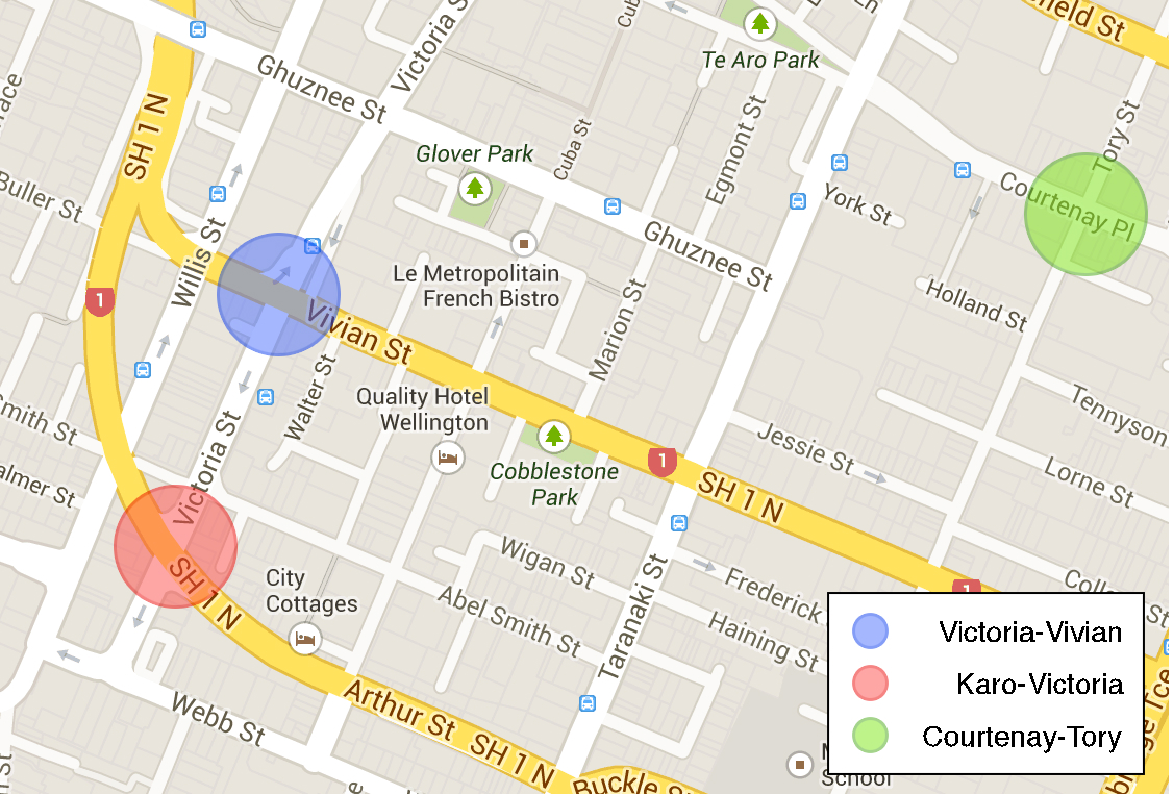
\includegraphics[scale=0.5]{intersection-map.pdf}
	\caption[A map of Wellington City showing intersections used for evaluation]{ A map of Wellington City showing the intersections of Vivian Street and Victoria Street, Courtenay Place and Tory Street, and Karo Drive and Victoria Street marked. }
\label{intersectionmap}
\end{figure}


\section{SCATS Representations} 

Figure \ref{scats_intersections} shows the three evaluation intersections used during evaluation of the PBTC system as represented in the SCATS system used by Wellington City Council. Screenshots were provided by Wellington City Council traffic engineers. The SCATS phase configuration for each intersection is shown to the left of each figure. Note that in the case of Courtenay-Tory, phases A, B, C, E, E1, and E2 are considered as a single phase in the SCATS log files and PBTSim configuration.


\begin{figure}[]
\centering
\begin{subfigure}{.5\textwidth}
  \centering
  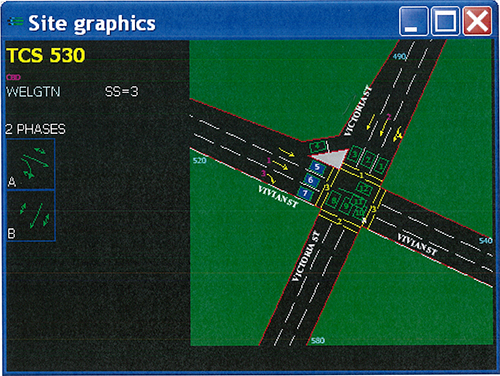
\includegraphics[scale=0.35]{scats-vivian-victoria.png}
  \caption{Vivian Street-Victoria Street}
  \label{fig:sub1}
\end{subfigure}%
\begin{subfigure}{.5\textwidth}
  \centering
  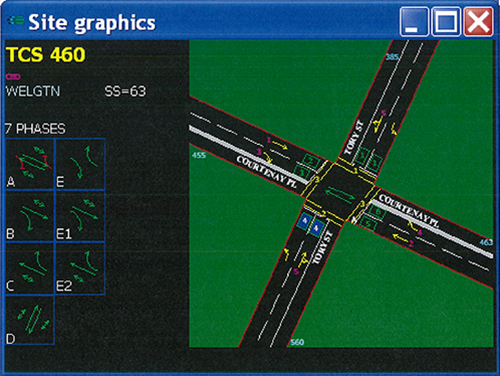
\includegraphics[scale=0.35]{scats-courtenay-tory.png}
  \caption{Courtenay Place-Tory Street}
  \label{fig:sub2}
\end{subfigure}

\vspace{1cm}

\begin{subfigure}{.5\textwidth}
  \centering
  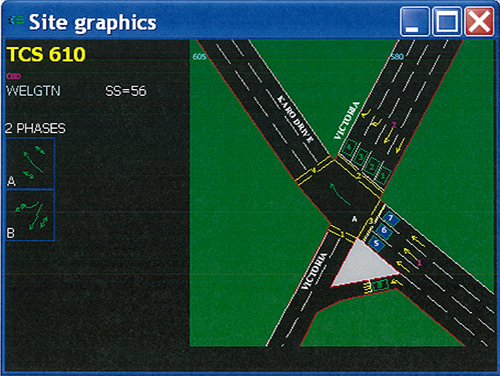
\includegraphics[scale=0.35]{scats-karo-victoria.png}
  \caption{Karo-Victoria}
  \label{fig:sub1}
\end{subfigure}%
\caption{ Screenshots of the Vivian-Victoria, Courtenay-Tory, and Karo-Victoria intersections as represented in the SCATS system. }
\label{scats_intersections}
\end{figure}

\section{PBTSim Representations}

Figure \ref{pbtsim_intersections} shows the visual representation of the three evaluation intersections within the PBTSim graphical user interface. All lanes catering for turning traffic have been omitted from each intersection and are not considered by this project. 

\begin{figure}[]
\centering
\begin{subfigure}{.5\textwidth}
  \centering
  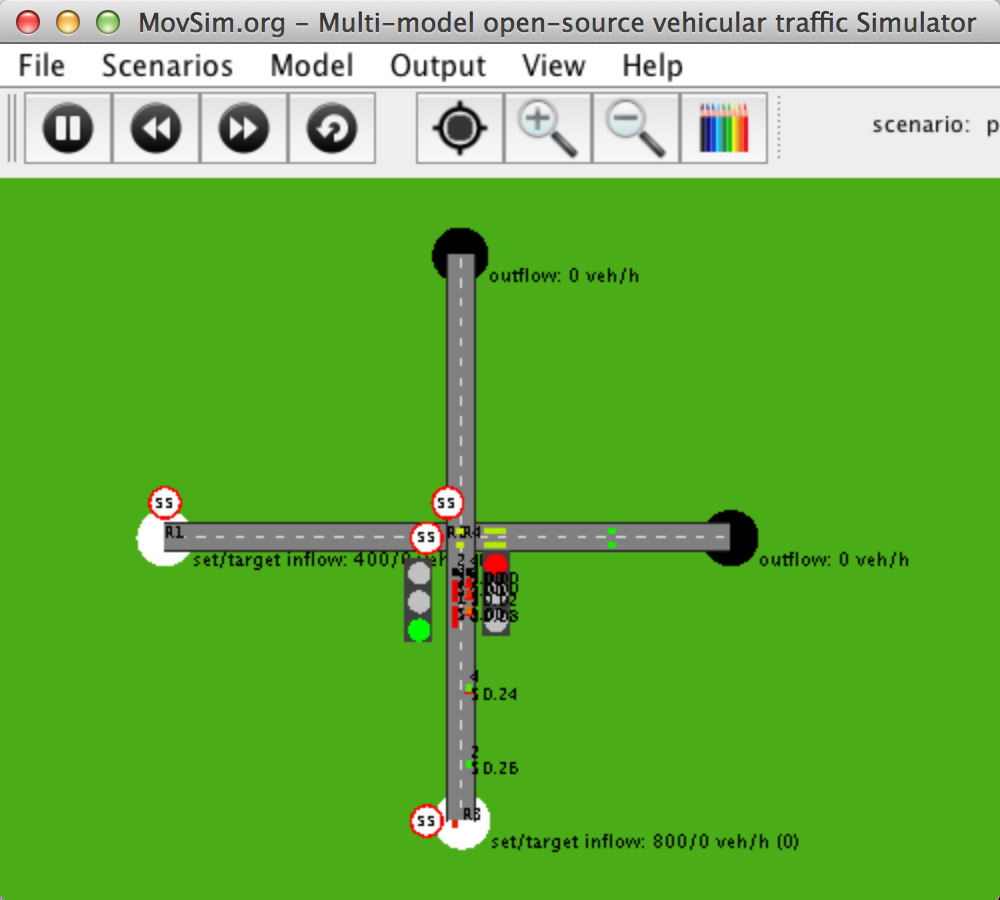
\includegraphics[scale=0.35]{pbtsim-vivian-victoria.png}
  \caption{Vivian-Victoria}
  \label{fig:sub1}
\end{subfigure}%
\begin{subfigure}{.5\textwidth}
  \centering
  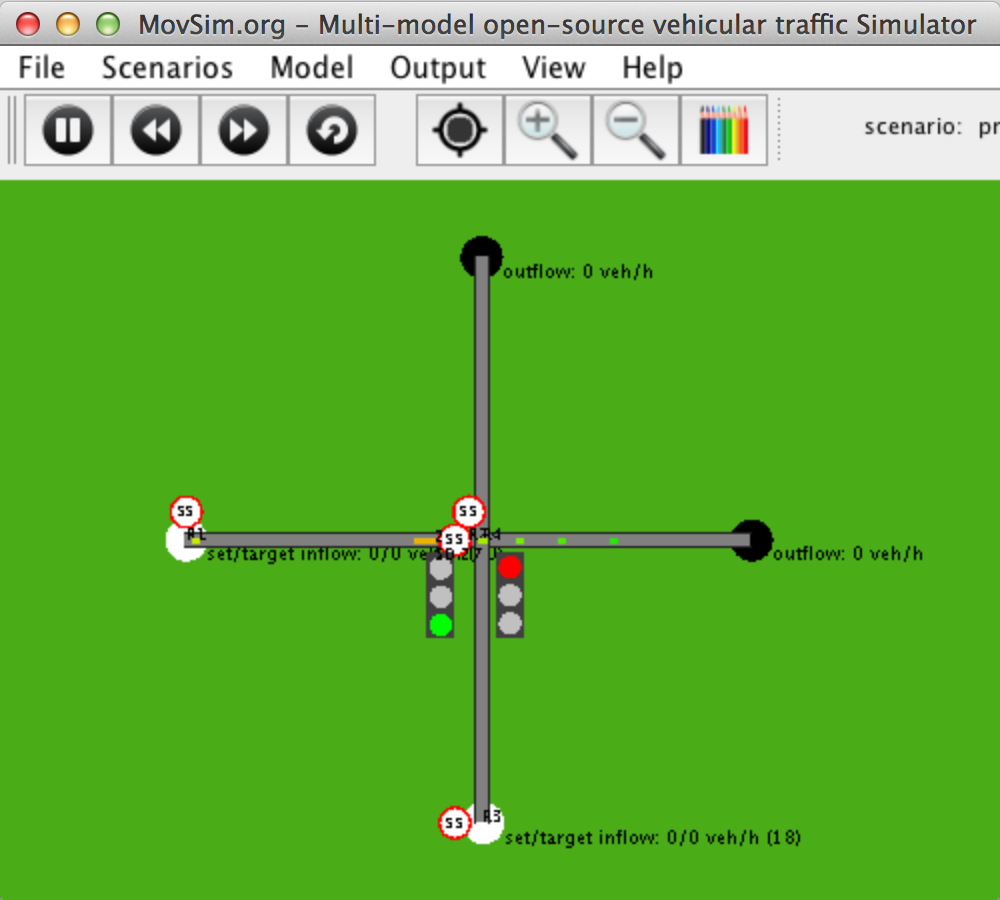
\includegraphics[scale=0.35]{pbtsim-courtenay-tory.png}
  \caption{Courtenay-Tory}
  \label{fig:sub2}
\end{subfigure}

\vspace{1cm}

\begin{subfigure}{.5\textwidth}
  \centering
  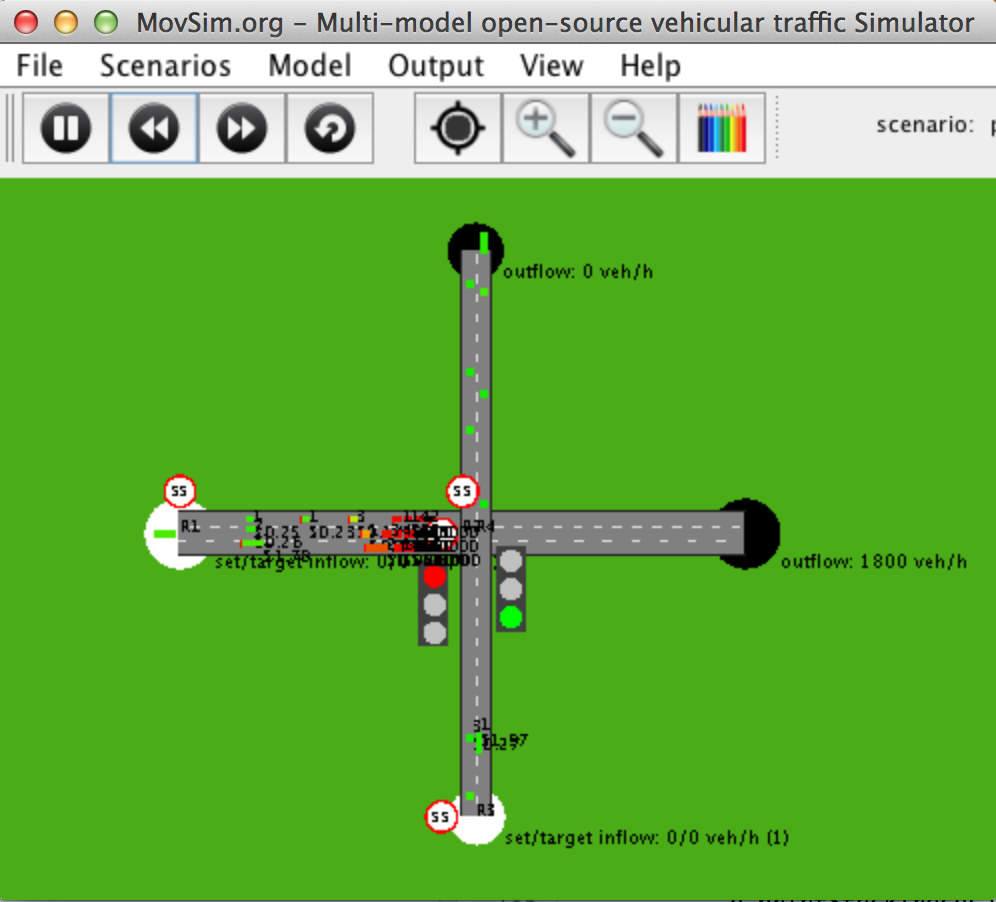
\includegraphics[scale=0.35]{pbtsim-karo-victoria.png}
  \caption{Karo-Victoria}
  \label{fig:sub1}
\end{subfigure}%
\caption[Screenshows of the Vivian-Victoria, Courtenay-Tory, and Karo-Victoria intersections as represented in the PBTSim simulator.]{ Intersections of Vivian-Victoria, Courtenay-Tory, and Karo-Victoria as represented in the PBTSim simulator.  }
\label{pbtsim_intersections}
\end{figure}

\end{appendices}


\end{document}
